\thispagestyle{thachthuctoanhocnone}
\pagestyle{thachthuctoanhoc}
\everymath{\color{thachthuctoanhoc}}
\graphicspath{{../thachthuctoanhoc/pic/}}
\begingroup
\AddToShipoutPicture*{\put(0,616){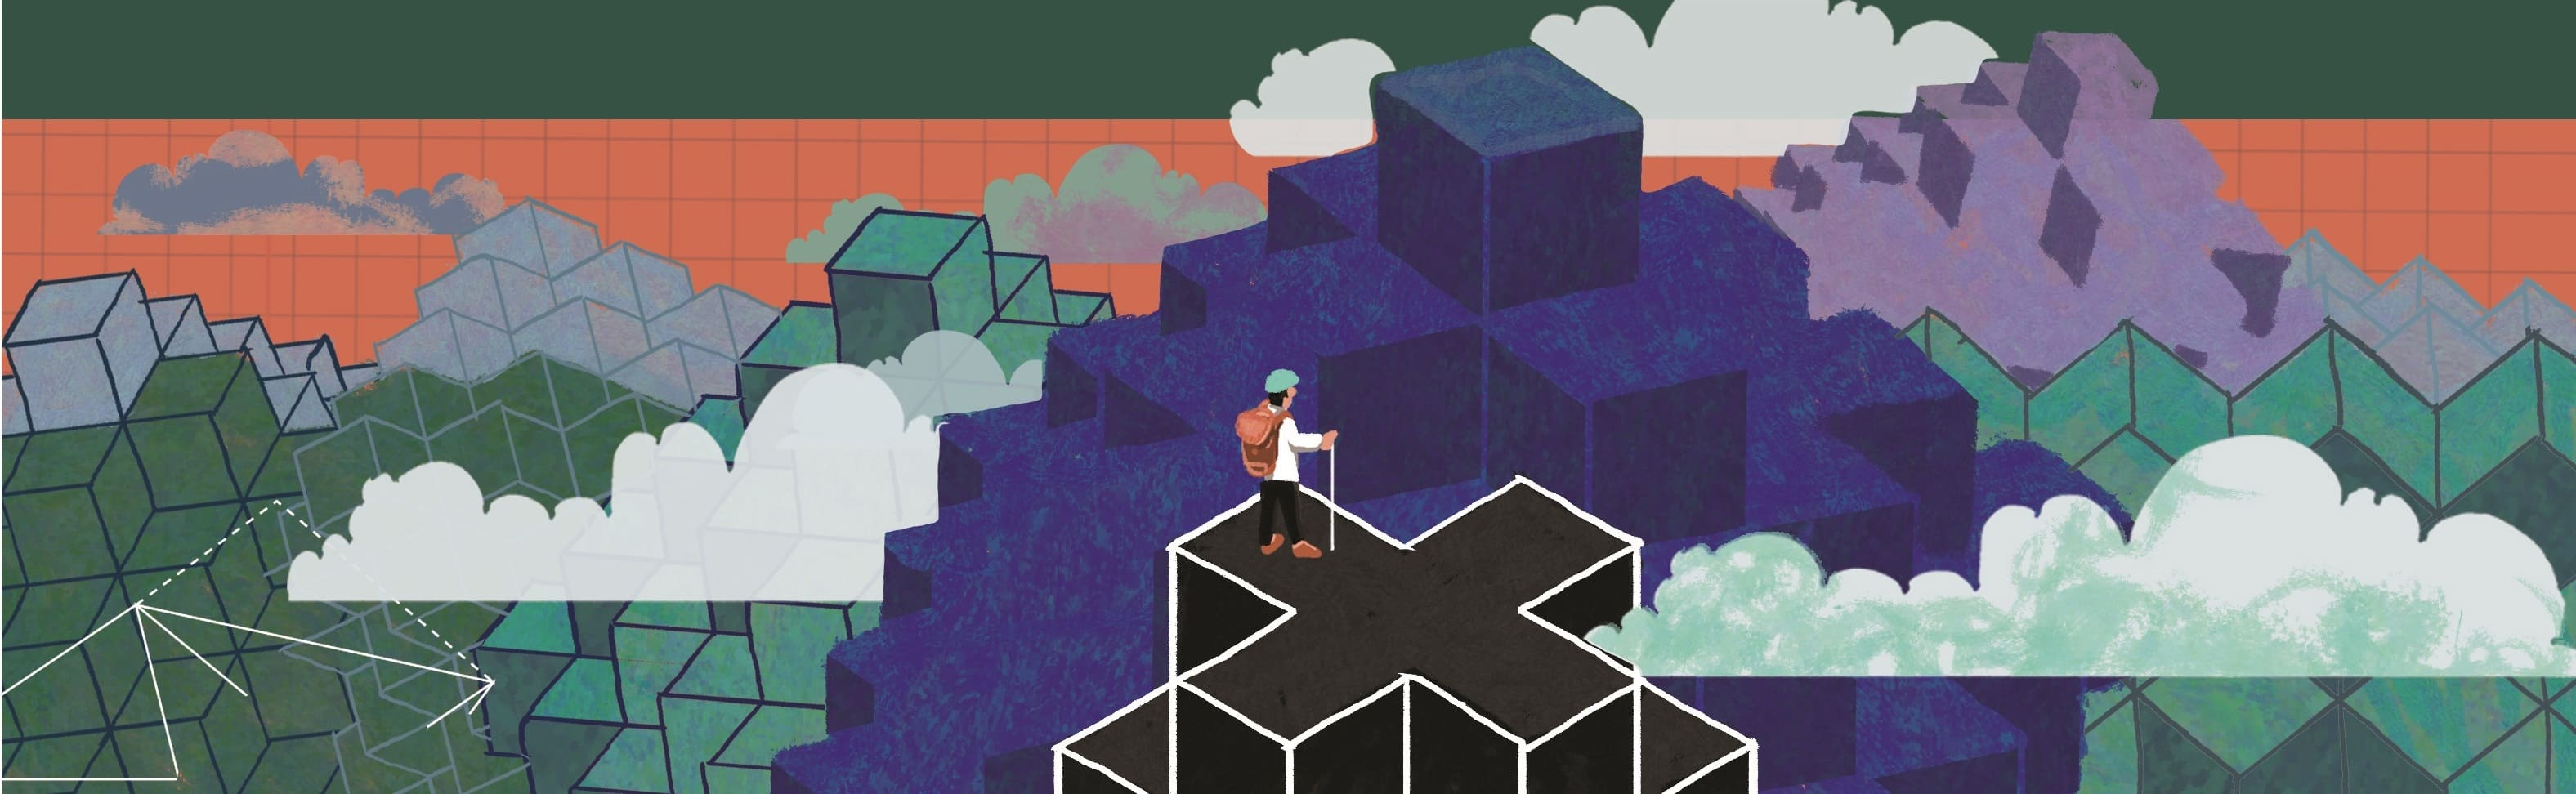
\includegraphics[width=19.3cm]{../thachthuctoanhoc/bannerthachthuc}}}
\centering
\vspace*{4cm}
\endgroup
\vspace*{-8pt}
\begin{tBox}
	\begin{itemize}[leftmargin = 13pt, itemsep = 1.0pt] 
		\item Mỗi bài toán đề xuất (kèm theo lời giải) cần được nêu rõ là bài sáng tác hay bài sưu tầm.
%				\item Mỗi bài toán đề xuất (kèm theo lời giải) cần được nêu rõ là bài sáng tác hay bài sưu tầm (nếu là bài sưu tầm, cần ghi rõ nguồn).
		\item Bài giải cho mỗi bài toán cần được trình bày trong một file riêng hoặc
		một tờ giấy riêng.
		\item  Người đề xuất bài toán hoặc gửi bài giải cho các bài toán trong mục ``Thách thức kỳ này" cần ghi rõ họ, đệm, tên và nơi làm việc/học tập, số điện thoại liên hệ. Nếu là học sinh (hoặc sinh viên) cần ghi rõ là học sinh lớp mấy (hoặc sinh viên năm thứ mấy).
		\item Các bài toán trong mục Thách thức kỳ này hướng tới các độc giả là học sinh phổ thông; được phân chia thành các mức độ $B$, $A$, và được sắp xếp theo độ khó tăng dần, theo đánh giá chủ quan của Ban biên tập. Các bài toán mức độ $B$ không đòi hỏi các kiến thức vượt quá chương trình môn Toán cấp THCS; các bài toán mức độ $A$ không đòi hỏi các kiến thức vượt quá chương trình môn Toán cấp THPT.
		\item Cách thức gửi bài toán đề xuất hoặc lời giải: gửi file thu được bằng cách scan, ảnh chụp (rõ nét) của bản viết tay, hoặc được soạn thảo bằng các phần mềm Latex, Word tới \url{bbt@pi.edu.vn} hoặc gửi qua đường bưu điện tới Tòa soạn (xem địa chỉ tại bìa $2$).
		\item Hạn gửi lời giải cho các bài toán P$691$--P$700$: trước ngày $15/5/2023$.
	\end{itemize}
\end{tBox}
\begin{center}
	\vspace*{-5pt}
	\textbf{\color{thachthuctoanhoc}\color{thachthuctoanhoc}\color{thachthuctoanhoc}THÁCH THỨC KỲ NÀY}
	\vspace*{-5pt}
\end{center}
\begin{multicols}{2}
	\setlength{\abovedisplayskip}{4pt}
	\setlength{\belowdisplayskip}{4pt}
	{\color{thachthuctoanhoc}{\usefont{T5}{qag}{b}{n} P691.}}
	(Mức $B$) Tìm tất cả các số có sáu chữ số, trong đó chữ số hàng trăm nghìn bằng $\dfrac16$ tổng năm chữ số còn lại; chữ số hàng chục nghìn bằng $\dfrac16$  tổng bốn chữ số nằm bên phải nó.
	\vskip 0.05cm
	\hfill	\textit{\small Duy Minh, Hà Nội (st)}
	\vskip 0.05cm
	{\color{thachthuctoanhoc}{\usefont{T5}{qag}{b}{n} P692.}}
	(Mức $B$)  Ở mỗi ô vuông con của bảng ô vuông kích thước $3\times3$, có $4$ viên bi. Bạn Hà lấy bi ra khỏi bảng, theo quy tắc: Mỗi lần, lấy hai viên bi nằm ở hai ô vuông con kề nhau, ở mỗi ô lấy một viên. Hỏi, bạn Hà có thể lấy ra khỏi bảng tối đa bao nhiêu viên bi?
	\vskip 0.05cm
	({\it Hai ô vuông được gọi là kề nhau, nếu chúng có cạnh chung}.)
	\begin{flushright}
		\textit{\small Trích Đề thi VMTC $2022$--Vòng $2$--Khối lớp $8$}
	\end{flushright}
	{\color{thachthuctoanhoc}{\usefont{T5}{qag}{b}{n} P693.}}
	(Mức $B$) Cho các số thực phân biệt $a,b,c$  thoả mãn
	\begin{align*}
		\dfrac{(a+b)(b+c)(c+a)}{(a-b)(b-c)(c-a)}=\dfrac{23}{20}.
	\end{align*}
	Tính
	\begin{align*}
		S=\dfrac{a}{a+b}+\dfrac{b}{b+c}+\dfrac{c}{c+a}.
	\end{align*}
	\begin{flushright}
		\textit{\small Trích Đề thi VMTC $2022$--Vòng $2$--Khối lớp $8$}
	\end{flushright}
	{\color{thachthuctoanhoc}{\usefont{T5}{qag}{b}{n} P694.}}
	(Mức $B$) Cho tập hợp $S$ gồm tất cả các số tự nhiên có ba chữ số. Chứng minh rằng, trong $106$ số đôi một khác nhau tùy ý thuộc $S$, luôn tồn tại $8$ số, sao cho có thể phân chia $8$ số này thành $4$ nhóm, mỗi nhóm có hai số, và các tổng hai số cùng nhóm bằng nhau.
	\begin{flushright}
		\textit{\small Trích Đề thi VMTC $2022$--Vòng $2$--Khối lớp $8$}
	\end{flushright}
	{\color{thachthuctoanhoc}{\usefont{T5}{qag}{b}{n} P695.}}
	(Mức $B$) Tìm tất cả các cặp số tự nhiên $(x;y)$ thoả mãn $x^2+16=5^y$. 
	\vskip 0.05cm
	\hfill\textit{\small Trích Đề thi VMTC $2022$--Vòng $2$--Khối lớp $9$}
	\vskip 0.05cm
	{\color{thachthuctoanhoc}{\usefont{T5}{qag}{b}{n} P696.}}
	(Mức $B$) Cho lục giác đều $ABCDEF$ có cạnh bằng $1$ và $M$ là một điểm tuỳ ý nằm trong lục giác đó. Chứng minh rằng, trong $6$ tam giác $MAB$, $MBC$, $MCD$, $MDE$, $MEF$ và $MFA$ có ít nhất $3$ tam giác có chu vi không nhỏ hơn $3$. 
	\begin{figure}[H]
		\vspace*{-15pt}
		\centering
		\captionsetup{labelformat= empty, justification=centering}
		\definecolor{qqzzff}{rgb}{0,0.6,1}
		\definecolor{zzttqq}{rgb}{0.6,0.2,0}
		\definecolor{qqqqff}{rgb}{0,0,1}
		\definecolor{qqqqffa}{rgb}{1,1,1}
		\begin{tikzpicture}[thachthuctoanhoc,scale=0.55]
			\draw [color=qqzzff] (-1.092089618842777,3.780911308935779)-- (2.5235020561954022,3.780911308935779);
			\draw [color=qqzzff] (2.5235020561954022,3.780911308935779)-- (4.331297893714492,6.912105549230374);
			\draw [color=qqzzff] (4.331297893714492,6.912105549230374)-- (2.5235020561954027,10.04329978952497);
			\draw [color=qqzzff] (2.5235020561954027,10.04329978952497)-- (-1.0920896188427762,10.04329978952497);
			\draw [color=qqzzff] (-1.0920896188427762,10.04329978952497)-- (-2.8998854563618672,6.912105549230376);
			\draw [color=qqzzff] (-2.8998854563618672,6.912105549230376)-- (-1.092089618842777,3.780911308935779);
			\draw  (-1.092089618842777,3.780911308935779)-- (0.9849524072429845,5.223301604828669);
			\draw  (0.9849524072429845,5.223301604828669)-- (2.5235020561954022,3.780911308935779);
			\draw  (0.9849524072429845,5.223301604828669)-- (4.331297893714492,6.912105549230374);
			\draw  (0.9849524072429845,5.223301604828669)-- (-2.8998854563618672,6.912105549230376);
			\draw  (0.9849524072429845,5.223301604828669)-- (-1.0920896188427762,10.04329978952497);
			\draw  (0.9849524072429845,5.223301604828669)-- (2.5235020561954027,10.04329978952497);
			\draw [fill=white] (-1.092089618842777,3.780911308935779) circle (1.5pt);
			\draw[color=qqqqff] (-1.284408324961828,3.1597447968988694) node {$A$};
			\draw [fill=white] (2.5235020561954022,3.780911308935779) circle (1.5pt);
			\draw[color=qqqqff] (2.523502056195404,3.15597447968988694) node {$B$};
			\draw [fill=white] (4.331297893714492,6.912105549230374) circle (1.5pt);
			\draw[color=qqqqff] (4.7500544082281167,7.079177118877521) node {$C$};
			\draw [fill=white] (2.5235020561954027,10.04329978952497) circle (1.5pt);
			\draw[color=qqqqff] (2.65812515047874,10.425522605349025) node {$D$};
			\draw [fill=white] (-1.0920896188427762,10.04329978952497) circle (1.5pt);
			\draw[color=qqqqff] (-1.284408324961828,10.425522605349025) node {$E$};
			\draw [fill=white] (-2.8998854563618672,6.912105549230376) circle (1.5pt);
			\draw[color=qqqqff] (-3.3037547392118753,7.002249636429901) node {$F$};
			\draw [fill=white] (0.9849524072429845,5.223301604828669) circle (1.5pt);
			\draw[color=qqqqff] (0.8887930541834608,4.681202135092791759) node {$M$};
		\end{tikzpicture}
		\vspace*{-15pt}
	\end{figure}
	\hfill	\textit{\small Nguyễn Văn Bản, Điện Biên}
	\vskip 0.05cm
	{\color{thachthuctoanhoc}{\usefont{T5}{qag}{b}{n} P697.}}
	(Mức $A$) Cho các số dương $x,y,z$ thoả mãn $x^2+y^2+z^2=3$. Chứng minh rằng
	\begin{align*}
		\sqrt[3]{\dfrac{y z}{x^5\!-\!x\!+\!8}}\!+\!\sqrt[3]{\dfrac{z x}{y^5\!-\!y\!+\!8}}\!+\!\sqrt[3]{\dfrac{x y}{z^5\!-\!z\!+\!8}} \!\le\! \dfrac{3}{2}.
	\end{align*}
	\hfill \textit{Hoàng Lê Nhật Tùng, Hà Nội}
	\vskip 0.05cm
	{\color{thachthuctoanhoc}{\usefont{T5}{qag}{b}{n} P698.}}
	(Mức $A$) Cho số nguyên $m>1$. Chứng minh rằng
	\vskip 0.05cm
	$a)$ Tồn tại $m$ số thực dương $x_1,\ldots,x_m$, không đồng thời bằng $1$, sao cho
	\begin{align*}
		\sqrt[n]{x_1}+\cdots+\sqrt[n]{x_m}
	\end{align*}
	là số nguyên, với mọi $n=1,2,\ldots,100$.
	\vskip 0.05cm
	$b)$ Không tồn  tại $m$ số thực dương $x_1,\ldots,x_m$, không đồng thời bằng $1$, sao cho
	\begin{align*}
		\sqrt[n]{x_1}+\cdots+\sqrt[n]{x_m}
	\end{align*}
	là số nguyên, với mọi số nguyên dương $n$.
	\vskip 0.05cm
	\hfill	\textit{\small Nguyễn Huy Hoàng, Bình Định}
	\vskip 0.05cm
	\columnbreak
	{\color{thachthuctoanhoc}{\usefont{T5}{qag}{b}{n} P699.}}
	(Mức $A$) Cho tam giác không cân $ABC$ nội tiếp đường tròn $(O)$ và có hai đường cao $BE,CF$ cắt nhau tại $H$. Giả sử   $\angle BAC$ khác $60^\circ,90^\circ$ và $120^\circ$.  Gọi $P, Q$ là các điểm, tương ứng, đối xứng với $B,C $ qua $F, E$. Các đường thẳng $HP, HQ$ theo thứ tự, tương ứng, cắt $AC, AB$ tại $M, N$.  Gọi $K$ là trung điểm của $BC$. Chứng minh rằng, các điểm $M, N, P, Q$ cùng thuộc một đường tròn có tâm nằm trên đường thẳng $HK$.
	\begin{figure}[H]
		\vspace*{-15pt}
		\centering
		\captionsetup{labelformat= empty, justification=centering}
		\definecolor{qqqqff}{rgb}{0,0,1}
		\definecolor{qqqqffa}{rgb}{1,1,1}
		\begin{tikzpicture}[thachthuctoanhoc,scale=0.65]
			\draw  (-0.27473499999999995,6.521887994397557) circle (3.8233413036603774cm);
			\draw  (-1.9190600551547001,9.973573645969253)-- (-3.68839,4.8);
			\draw  (-3.68839,4.8)-- (3.13892,4.8);
			\draw  (3.13892,4.8)-- (-1.9190600551547001,9.973573645969253);
			\draw  (-3.68839,4.8)-- (-0.19761156573467797,8.212783678306042);
			\draw  (-2.973484746555942,6.8904043303842535)-- (3.13892,4.8);
			\draw  (-3.534143131469356,11.625567356612084)-- (-1.9190600551547001,9.973573645969253);
			\draw  (-2.474847925491419,10.542063329077637)-- (-1.919060055154701,6.529797657174141);
			\draw  (-3.534143131469356,11.625567356612084)-- (-1.919060055154701,6.529797657174141);
			\draw [dashed] (-4.685663359168936,9.440209986300777) circle (2.47017927907576cm);
			\draw [dashed] (-4.685663359168939,9.44020998630077)-- (-0.27473499999999995,4.8);
			\draw [fill=white] (-1.9190600551547001,9.973573645969253) circle (1.5pt);
			\draw[color=qqqqff] (-1.72146890661847,10.48321821718474) node {$A$};
			\draw [fill=white] (-3.68839,4.8) circle (1.5pt);
			\draw[color=qqqqff] (-4.0153339518523685,4.579033939329845) node {$B$};
			\draw [fill=white] (3.13892,4.8) circle (1.5pt);
			\draw[color=qqqqff] (3.3889362337311386,4.579033939329845) node {$C$};
			\draw [fill=white] (-0.19761156573467797,8.212783678306042) circle (1.5pt);
			\draw[color=qqqqff] (0.13433673518798938,8.502335544158505) node {$E$};
			\draw [fill=white] (-2.973484746555942,6.8904043303842535) circle (1.5pt);
			\draw[color=qqqqff] (-3.3037547392118753,7.04071337765371) node {$F$};
			\draw [fill=white] (-1.919060055154701,6.529797657174141) circle (1.5pt);
			\draw[color=qqqqff] (-2.1113787612737522,5.8974811953692) node {$H$};
			\draw [fill=white] (-2.258579493111884,8.980808660768506) circle (1.5pt);
			\draw[color=qqqqff] (-1.9575237963785104,8.944668568232325) node {$P$};
			\draw [fill=white] (-3.534143131469356,11.625567356612084) circle (1.5pt);
			\draw[color=qqqqff] (-3.2691602808380743,12.098695348584778) node {$Q$};
			\draw [fill=white] (-2.474847925491419,10.542063329077637) circle (1.5pt);
			\draw[color=qqqqff] (-2.1229293380047094,10.84862375881094) node {$M$};
			\draw [fill=white] (-2.48555043367752,8.31713884614052) circle (1.5pt);
			\draw[color=qqqqff] (-2.8806535857499607,8.4831036735466) node {$N$};
			\draw [fill=white] (-0.27473499999999995,6.521887994397557) circle (1.5pt);
			\draw[color=qqqqff] (-0.11126421763561023,6.829162800922753) node {$O$};
			\draw [fill=white] (-0.27473499999999995,4.8) circle (1.5pt);
			\draw[color=qqqqff] (-0.3420466649784728,4.252133832749413) node {$K$};
			\draw [fill=white] (-4.685663359168939,9.44020998630077) circle (1.5pt);
		\end{tikzpicture}
		\vspace*{-20pt}
	\end{figure}
	\hfill	\textit{\small Lưu Công Đông, Hà Nội}
	\vskip 0.05cm
	{\color{thachthuctoanhoc}{\usefont{T5}{qag}{b}{n} P700.}}
	(Mức $A$) Cho số nguyên dương $n$. Lần lượt ghi các số $n^3,$ $n^3+1,\ldots,$ $n^3+n$ lên $n+1$ tấm thẻ trắng, trên mỗi thẻ ghi đúng một số. Người ta xếp tất cả $n+1$ tấm thẻ đó vào hai chiếc hộp xanh và đỏ, sao cho mỗi hộp có ít nhất một thẻ và  tổng các số được ghi ở các thẻ trong hộp xanh chia hết cho tổng các số được ghi ở các thẻ trong hộp đỏ. Chứng minh rằng, số các tấm thẻ trong hộp xanh chia hết cho số các tấm thẻ trong hộp đỏ.
	\vskip 0.05cm
	\hfill	\textit{\small Tô Trung Hiếu, Nghệ An (st)}
\end{multicols}
\centerline{{\large{\textbf{\color{thachthuctoanhoc}GIẢI BÀI KỲ TRƯỚC}}}}
\vspace*{-5pt}
\begin{multicols}{2}
	\setlength{\abovedisplayskip}{4pt}
	\setlength{\belowdisplayskip}{4pt}
	{\color{thachthuctoanhoc}{\usefont{T5}{qag}{b}{n} P661.}}
	(Mức $B$) Một xấp tiền giấy có $120$ tờ tiền, gồm các tờ tiền với mệnh giá $10{.}000$ đồng, $50{.}000$ đồng, và $100{.}000$ đồng. Số tờ tiền mệnh giá $50{.}000$ đồng là một số lớn hơn $5$ và chia hết cho $5$. Hỏi mỗi loại mệnh giá có bao nhiêu tờ tiền? Biết rằng, tổng mệnh giá của cả xấp tiền là $8{.}600{.}000$ đồng.\\
	\textbf{\color{thachthuctoanhoc}Lời giải} (\textit{dựa theo lời giải của tác giả bài toán})\textbf{\color{thachthuctoanhoc}.}\\
	Giả sử $x$, $y$, $z$ tương ứng là số tờ tiền mệnh giá $10{.}000$ đồng, $50{.}000$ đồng, $100{.}000$ đồng.
	\vskip 0.01cm
	Theo các giả thiết của bài ra, ta có:
	\begin{align*}
		x,y,z \in \mathbb{N^*}, y > 5, y \text{ chia hết cho } 5, \text{ và}
	\end{align*}
	\begin{align*}
		\begin{cases}
			x + y + z = 120  \hspace*{102pt} {\color{black}(}1{\color{black})} \\[-0.5ex]
			(x + 5y + 10z) \cdot 10^4 = 860 \cdot 10^4.\hspace*{24pt} {\color{black}(}2{\color{black})} 
		\end{cases}
	\end{align*}
	Từ ($2$), ta được:
	\begin{align*}
		x + 5y + 10z = 860. \tag{$3$}
	\end{align*}
	Từ ($1$) và ($3$), suy ra
	\begin{align*}
		4y + 9z = 740;
	\end{align*}
	do đó, $4(185-y)= 9z$. \hfill ($4$)
	\vskip 0.05cm
	Vì $z$ là số nguyên và $(4, 9) = 1$ nên từ ($4$) suy ra, $185 - y$ chia hết cho $9$. Mà $185$ chia $9$ dư $5$, nên $y$ chia $9$ dư $5$. Do đó
	\begin{align*}
		y = 9t + 5,  \tag{$5$}
	\end{align*}
	với $t$ là một số nguyên dương (vì $y > 5$).
	\vskip 0.05cm
	Vì $y$ chia hết cho $5$ nên từ ($5$) suy ra, $9t$ chia hết cho $5$.
	\vskip 0.05cm
	Mà $(9, 5) = 1$ nên $t$ chia hết cho $5$.       \hfill           ($6$)
	\vskip 0.05cm
	Thay ($5$) vào ($4$), ta được:
	\begin{align*}
		36\left( {20 - t} \right) = 9z;
	\end{align*}
	suy ra, $z = 80 - 4t$. \hfill ($7$)
	\vskip 0.05cm
	Thay ($5$) và ($7$) vào ($3$), ta được:
	\begin{align*}
		x + 5t + 825 = 860;
	\end{align*}
	suy ra,  $x = 5 (7-t)$ \hfill ($8$)
	\vskip 0.05cm
	Vì $x > 0$ nên từ ($8$) và ($6$), với lưu ý $t \in \mathbb{N^*}$,  suy ra $t = 5$. Vì vậy, từ ($8$), ($5$) và ($7$), ta được $x = 10$, $y = 50$, $z = 60$.
	\vskip 0.05cm
	Ngược lại, với $x, y, z$ là các số vừa nêu trên, ta có $y$ lớn hơn $5$, chia hết cho $5$, và
	\begin{align*}
		\begin{cases}
			x + y + z = 120\\[-0.5ex]
			(x + 5y + 10z) \cdot 10^4 = 860 \cdot 10^4.
		\end{cases}
	\end{align*}
	Vậy, số tờ tiền mệnh giá $10{.}000$ đồng, $50{.}000$ đồng, $100{.}000$ đồng, tương ứng, là $10$ tờ, $50$ tờ, $60$ tờ.
	\vskip 0.05cm
	\textbf{\color{thachthuctoanhoc}Bình luận và Nhận xét}
	\vskip 0.05cm	
	$\pmb{1.}$ Để thuận tiện cho việc theo dõi lời giải của đông đảo đối tượng bạn đọc, trong lời giải trên, chúng tôi đã không sử dụng các ký hiệu của phép chia hết và phép đồng dư.
	\vskip 0.05cm
	$\pmb{2.}$ Trong số các bạn đọc đã gửi lời giải tới Tạp chí, một số bạn cho kết quả sai, do \textit{không} lưu ý tới giả thiết ``số tờ tiền mệnh giá $50{.}000$ đồng là một số lớn hơn $5$".
	\vskip 0.05cm
	\hfill	\textbf{\color{thachthuctoanhoc}Lê Huy}
	\vskip 0.05cm
	{\color{thachthuctoanhoc}{\usefont{T5}{qag}{b}{n} P662.}}
	(Mức $B$) Với mỗi số thực $x$, đặt $f(x)=\sqrt[3]{x^3-x}$. Cho các số thực đôi một phân biệt $a,b,c$ thoả mãn
	\begin{align*}
		&a f(b)+b f(c)+c f(a)\\[-0.5ex]
		=\,\,&a f(c)+b f(a)+c f(b)=0.
	\end{align*}
	Chứng minh rằng $a+b+c=0$. 
	\vskip 0.05cm
	\textbf{\color{thachthuctoanhoc}Lời giải} (\textit{dựa theo đa số lời giải Tạp chí nhận được từ bạn đọc})\textbf{\color{thachthuctoanhoc}.}
	\vskip 0.05cm
	Trước hết, ta nhắc lại (không chứng minh) kết quả rất quen thuộc sau:
	\vskip 0.05cm
	\textit{Nhận xét.} Với $x, y, z$ là ba số thực: 
	\begin{align*}
		\text{Nếu } x + y + z = 0 \text{ thì } {x^3} + {y^3} + {z^3} = 3xyz.   
	\end{align*}
	Theo Nhận xét trên, vì $af\left( b \right) + bf\left( c \right) + cf\left( a \right) = 0$  nên
	\begin{align*}
		&{a^3}{\left( {f\left( b \right)} \right)^3} + {b^3}{\left( {f\left( c \right)} \right)^3} + {c^3}{\left( {f\left( a \right)} \right)^3} \\[-0.5ex]
		= \,\,&abc \cdot f\left( a \right)f\left( b \right)f\left( c \right);
	\end{align*}
	và vì $af\left( c \right) + bf\left( a \right) + cf\left( b \right) = 0$  nên 
	\begin{align*}
		&{a^3}{\left( {f\left( c \right)} \right)^3} + {b^3}{\left( {f\left( a \right)} \right)^3} + {c^3}{\left( {f\left( b \right)} \right)^3} \\[-0.5ex]
		=\,\,& abc \cdot f\left( a \right)f\left( b \right)f\left( c \right).
	\end{align*}
	Suy ra
	\begin{align*}
		&{a^3}{\left( {f\left( b \right)} \right)^3} + {b^3}{\left( {f\left( c \right)} \right)^3} + {c^3}{\left( {f\left( a \right)} \right)^3}\\[-0.5ex]
		 = \,\,&{a^3}{\left( {f\!\left(c \right)} \!\right)^3} \!+\! {b^3}{\left(\! {f\!\left( a \right)} \!\right)^3} \!+\! {c^3}{\left(\! {f\left( b \right)} \!\right)^3}. \tag{$*$}
	\end{align*}
	Ta có:
	\begin{align*}
		&(*) \\
		\Leftrightarrow&\, {a^3}\left( {{b^3} - b} \right) + {b^3}\left( {{c^3} - c} \right) + {c^3}\left( {{a^3} - a} \right) \\[-0.6ex]
		&= {a^3}( {{c^3} - c}) + {b^3}( {{a^3} - a} ) + {c^3}( {{b^3} - b})\\[-0.6ex]
		\Leftrightarrow&\, {a^3}c - {c^3}a + {c^3}b - {a^3}b + {b^3}a - {b^3}c = 0\\[-0.6ex]
		\Leftrightarrow&\, ac( {{a^2} \!-\! {c^2}} ) \!-\! b( {{a^3} \!-\! {c^3}}) \!+\! {b^3}( {a \!-\! c} ) \!=\! 0\\[-0.6ex]
		\Leftrightarrow& ( \!{a \!-\! c}\!)\!(\! {{a^2}c \!+\! a{c^2} \!-\! {a^2}b \!-\! abc \!-\! b{c^2} \!+\! {b^3}} \!) \!=\! 0\\[-0.6ex]
%		\end{align*}
%		\begin{align*}
		\Leftrightarrow &(\! {a \!-\! c}\!)\!(\! {a^2}( {c \!-\! b}\! ) \!+\! ac(\! {c \!-\! b} \!) \!-\! b(\! {{c^2} \!-\! {b^2}}\!)\!) \!=\! 0\\[-0.6ex]
		\Leftrightarrow& \left( {a - c} \right)\left( {c - b} \right)\left( {{a^2} + ac - bc - {b^2}} \right) = 0\\[-0.6ex]
		\Leftrightarrow& \left( {a - c} \right)\left( {c - b} \right)\left( {a - b} \right)\left( {a + b + c} \right) = 0\\[-0.6ex]
		\Leftrightarrow& \,a \!+\! b \!+\! c \!=\! 0 \text{ (do $a,b,c$ đôi một phân biệt).}
	\end{align*}
	Ta có điều phải chứng minh theo yêu cầu đề bài.
	\vskip 0.05cm
	\textbf{\color{thachthuctoanhoc}Bình luận và Nhận xét}
	\vskip 0.05cm
	Rất tiếc, trong số các lời giải Tạp chí đã nhận được từ bạn đọc, có hai lời giải sai, do người giải bài đã \textit{ngộ nhận} rằng, với giả thiết $a + b + c \ne 0$, ta có:
	\begin{align*}
		&f\left( a \right) + f\left( b \right) + f\left( c \right) \\[-0.5ex]
		&= \dfrac{a}{{a + b + c}}f\left( a \right) + \dfrac{b}{{a + b + c}}f\left( b \right) \\[-0.5ex]
		&\quad+ \dfrac{c}{{a + b + c}}f\left( c \right)\\[-0.5ex]
		\Leftrightarrow &\dfrac{a}{{a + b + c}} = \dfrac{b}{{a + b + c}} = \dfrac{c}{{a + b + c}} = 1.
	\end{align*}
	\hfill	\textbf{\color{thachthuctoanhoc}Lưu Thị Thanh Hà}
	\vskip 0.05cm
	{\color{thachthuctoanhoc}{\usefont{T5}{qag}{b}{n} P663.}}
	(Mức $B$) Cho hai đường tròn đồng tâm $(C_1)$ và $(C_2)$, có bán kính, tương ứng, là $14$ và $50$. Tìm số nguyên dương $k$ nhỏ nhất có tính chất: Nếu qua một điểm tuỳ ý nằm trên $(C_1)$, kẻ $k$ dây cung tuỳ ý của $(C_2)$ thì chắc chắn có một dây cung có độ dài không nguyên. 
	\vskip 0.05cm
	\textbf{\color{thachthuctoanhoc}Lời giải} (\textit{dựa theo lời giải của bạn Trần Minh Hoàng, lớp 10T1, trường THPT chuyên Hà Tĩnh, tỉnh Hà Tĩnh})\textbf{\color{thachthuctoanhoc}.}
	\vskip 0.05cm
	Gọi $O$ là tâm chung của hai đường tròn $(C_1)$ và $(C_2)$.
	\vskip 0.05cm 
	Xét điểm $M$ tùy ý nằm trên  $(C_1)$; và xét dây $AB$ tùy ý của $(C_2)$, đi qua $M$. Xảy ra các trường hợp sau:
	\vskip 0.05cm
	$\diamond$ \textit{Trường hợp} $1$: $AB$ tiếp xúc với  $(C_1)$ tại $M$ (xem Hình $1$).
	\begin{figure}[H]
		\vspace*{-15pt}
		\centering
		\captionsetup{labelformat= empty, justification=centering}
		\definecolor{qqwuqq}{rgb}{0.,0.39215686274509803,0.}
		\definecolor{ubqqys}{rgb}{0.29411764705882354,0.,0.5098039215686274}
		\begin{tikzpicture}[thachthuctoanhoc,scale=0.6]
			\draw[color=qqwuqq] (-0.11762822976546994,0.5713371160037106) -- (0.13377857056640663,0.62309733960145) -- (0.08201834696866722,0.8745041399333265) -- (-0.1693884533632093,0.8227439163355872) -- cycle; 
			\draw  (0.,0.) circle (3.cm);
			\draw  (0.,0.) circle (0.84cm);
			\draw  (0.,0.)-- (-0.1693884533632093,0.8227439163355872);
			\draw (0.7352,0.1878) node[anchor=north west] {$(C_1)$};
			\draw (3.01,0.2604) node[anchor=north west] {$(C_2)$};
			\draw  (-2.9902247379423654,0.2419835048045842)-- (2.6514478312159473,1.403504327866591);
			\draw  (0.,0.)-- (-2.9902247379423654,0.2419835048045842);
				\draw [fill=white] (0.,0.) circle (1.5pt);
				\draw (0.1302,-0.389) node {$O$};
				\draw [fill=white] (-0.1693884533632093,0.8227439163355872) circle (1.5pt);
				\draw (-0.4022,1.1921) node {$M$};
				\draw [fill=white] (-2.9902247379423654,0.2419835048045842) circle (1.5pt);
				\draw (-3.4578,0.2725) node {$A$};
				\draw [fill=white] (2.6514478312159473,1.403504327866591) circle (1.5pt);
				\draw (2.99438,1.7003) node {$B$};
		\end{tikzpicture}
		\caption{\small\textit{\color{thachthuctoanhoc}Hình $1$}}
		\vspace*{-15pt}
	\end{figure}
	Khi đó, $OM \bot AB$ và do đó, $M$ là trung điểm của $AB$. Vì thế
	\begin{align*}
		AB &= 2AM = 2\sqrt {O{A^2} - O{M^2}}  \\
		&= 2\sqrt {{{50}^2} - {{14}^2}}  = 96 \in \mathbb{Z}.
	\end{align*}
	$\diamond$ \textit{Trường hợp} $2$: $AB$ cắt  $(C_1)$ và đi qua $O$.
	\vskip 0.05cm
	Trong trường hợp này, $AB$ là đường kính của $(C_2).$ Do đó
	\begin{align*}
		AB = 2 \cdot 50 = 100 \in \mathbb{Z}.
	\end{align*}
	$\diamond$ \textit{Trường hợp} $3$: $AB$ cắt $(C_1)$ và không đi qua $O$ (xem Hình $2$).
	\begin{figure}[H]
		\vspace*{-15pt}
		\centering
		\captionsetup{labelformat= empty, justification=centering}
		\definecolor{qqwuqq}{rgb}{0.,0.39215686274509803,0.}
		\definecolor{ubqqys}{rgb}{0.29411764705882354,0.,0.5098039215686274}
		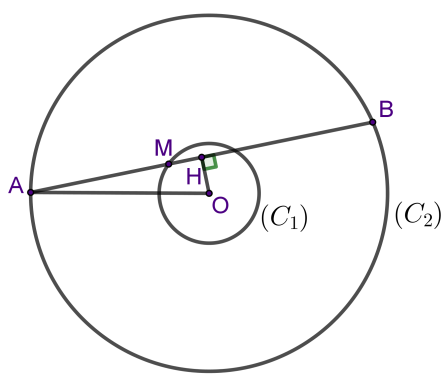
\includegraphics[width=0.7\linewidth]{P663H2}
		\caption{\small\textit{\color{thachthuctoanhoc}Hình $2$}}
		\vspace*{-10pt}
	\end{figure}
	Gọi $H$ trung điểm của $AB$; ta có, $OH \bot AB$. Do đó, $AB$ tiếp xúc với đường tròn tâm $O$, bán kính $OH$, và
	\begin{align*}
		AB = 2AM = 2\sqrt {O{A^2} - O{H^2}}. \tag{$1$}
	\end{align*}
	Do $0 < OH < OM$, từ ($1$) suy ra
	\begin{align*}
		96 &= 2\sqrt {O{A^2} - O{M^2}}  < AB < 2\sqrt {O{A^2}}  \\
		&= 2\sqrt {{{50}^2}}  = 100.
	\end{align*}
	Vì thế, độ dài $AB$ là số nguyên khi và chỉ khi $AB \in \{97; 98; 99\}$.
	\vskip 0.05cm
	Từ ($1$) ta có:
	\vskip 0.05cm
	$+$ $AB = 97  \Leftrightarrow  OH = \dfrac{{\sqrt {591} }}{2}$;
	\vskip 0.05cm
	$+$ $AB = 98  \Leftrightarrow OH = 3\sqrt{11}$;
	\vskip 0.05cm
	$+$ $AB = 99  \Leftrightarrow  OH = \dfrac{{\sqrt {199} }}{2}$.
	\vskip 0.05cm
	Vì vậy, trong trường hợp này, độ dài dây $AB$ là số nguyên khi và chỉ khi dây $AB$ đi qua $M$ và tiếp xúc với một trong các đường tròn $\left( {O,\frac{{\sqrt {591} }}{2}} \right),$    $\left( {O,3\sqrt {11} } \right),$      $\left( {O,\frac{{\sqrt {199} }}{2}}\right)$. \hfill ($2$)
	\vskip 0.05cm
	Dễ thấy, $\dfrac{{\sqrt {591} }}{2},3\sqrt {11} ,\dfrac{{\sqrt {199} }}{2} < 14 = OM;$  do đó, $M$ nằm ngoài cả ba đường tròn vừa nêu trên. Vì thế, với mỗi đường tròn, trong ba đường tròn đó, sẽ có đúng hai dây của  $(C_2)$ đi qua $M$ và tiếp xúc đường tròn ấy.                  \hfill ($3$)
	\vskip 0.05cm
	Vì ba đường tròn được nêu ở ($2$) đồng tâm, nên không có hai đường tròn nào trong chúng có tiếp tuyến chung. Do đó, từ ($2$) và ($3$) suy ra, có $2 \cdot 3 = 6$  dây của  $(C_2)$ đi qua $M$ và có độ dài nguyên.
	\vskip 0.05cm
	Từ kết quả xét ba trường hợp trên, suy ra, với mỗi điểm $M$ nằm trên $(C_1)$  có đúng $1 + 1 + 6 = 8$ dây của $(C_2)$  đi qua $M$ và có độ dài nguyên. Vì thế, số nguyên dương $k$ nhỏ nhất, thỏa mãn yêu cầu đề bài, bằng $9$.
	\vskip 0.05cm
	\textbf{\color{thachthuctoanhoc}Bình luận và Nhận xét}
	\vskip 0.05cm
	Trong số các lời giải Tạp chí đã nhận được từ bạn đọc, lời giải của bạn \textit{Trần Minh Hoàng} là lời giải duy nhất đúng và hoàn chỉnh. Trong số các lời giải còn lại:
	\vskip 0.05cm
	-- Có \textit{hai lời giải không được chấp nhận là lời giải hoàn chỉnh}, do người giải bài chỉ liệt kê các khẳng định mang tính mấu chốt, mà không có bất kỳ sự giải thích nào cho tính đúng của các khẳng định đó;
	\vskip 0.05cm
	-- Có \textit{ba lời giải sai}, do người giải bài đã mắc một trong các lỗi sau:
	\vskip 0.05cm
	+ Nhầm lẫn một điều kiện cần thành điều kiện cần và đủ;
	\vskip 0.05cm
	+ Giải một bài toán hoàn toàn khác, không liên quan một chút nào với bài đã ra.
	\vskip 0.05cm
	\hfill	\textbf{\color{thachthuctoanhoc}Hà Thanh}
	\vskip 0.05cm
	{\color{thachthuctoanhoc}{\usefont{T5}{qag}{b}{n} P664.}}
	(Mức $B$) Giải hệ phương trình
	\begin{align*}
		\begin{cases}
			x^{23}=3y^{21}-2z^{19}&\\[-0.5ex]
			y^{23}=3z^{21}-2x^{19}&\\[-0.5ex]
			z^{23}=3x^{21}-2y^{19}.
		\end{cases}
	\end{align*}
	\textbf{\color{thachthuctoanhoc}Lời giải} (\textit{dựa theo đa số lời giải Tạp chí nhận được từ bạn đọc})\textbf{\color{thachthuctoanhoc}.}
	\vskip 0.05cm
	$\bullet$ Giả sử $(x, y, z)$ là một nghiệm của hệ phương trình đã cho.
	\vskip 0.05cm
	Vì tính đối xứng vòng quanh của hệ đã cho đối với $x, y, z$, nên không mất tính tổng quát, có thể giả sử $x = \max\{x, y, z\}$ (tức, giả sử $x \ge y$ và $x \ge z$).
	\vskip 0.05cm
	Khi đó, ta có ${x^{23}} \ge {z^{23}};$ vì thế, từ phương trình thứ nhất và phương trình thứ ba của hệ đã cho, ta được:
	\begin{align*}
		3{y^{21}} - 2{z^{19}} \ge 3{x^{21}} - 2{y^{19}}.
	\end{align*}
	Do đó 
	\begin{align*}
		&2{y^{19}} - 2{z^{19}} \ge 3{x^{21}} - 3{y^{21}} \ge 0 \\[-0.5ex]
		&\text{ (do từ } x \ge y \text{ suy ra } x^{21} \ge y^{21});
	\end{align*}
	suy ra, $y \ge z$. Do đó,  $y^{23} \ge z^{23}$; vì thế, từ phương trình thứ hai và phương trình thứ ba của hệ đã cho, ta được:
	\begin{align*}
		3{z^{21}} - 2{x^{19}} \ge 3{x^{21}} - 2{y^{19}}.
	\end{align*}
	Do đó
	\begin{align*}
		&2{y^{19}} - 2{z^{19}} \ge 3{x^{21}} - 3{y^{21}} \ge 0 \\[-0.5ex]
		&\text{(do từ } x \ge y \text{ suy ra } x^{21} \ge y^{21}); \tag{$1$}
	\end{align*}
	suy ra, $y \ge x$. Mà $x \ge y$ nên $x = y$.  \hfill ($2$)
	\vskip 0.05cm
	Vì thế, từ ($1$) ta có:
	\begin{align*}
		0 \ge 3{x^{21}} - 3{z^{21}} \ge 0;
	\end{align*}
	suy ra, $3{x^{21}} - 3{z^{21}} = 0$; do đó, $x = z$. \hfill ($3$)
	\vskip 0.05cm
	Từ ($2$) và ($3$) suy ra, $x = y = z$.
	\vskip 0.05cm
	Thế $y = x$ và $z = x$ vào phương trình thứ nhất của hệ đã cho, ta được:
	\begin{align*}
		{x^{23}} = 3{x^{21}} - 2{x^{19}}. \tag{$4$}
	\end{align*}
	Ta có:
	\begin{align*}
		(4) \Leftrightarrow& {x^{19}}\left( {{x^4} - 3{x^2} + 2} \right) = 0\\[-0.5ex]
			\Leftrightarrow &{x^{19}}\left( {{x^2} - 1} \right)\left( {{x^2} - 2} \right) = 0\\[-0.5ex]
			\Leftrightarrow & x = 0,x =  \pm 1,x =  \pm \sqrt 2 .
	\end{align*}
	Như vậy, nếu $(x, y, z)$ là nghiệm của hệ đã cho thì
	\begin{align*}
		\left( {x,y,z} \right) \in &\left\{\!\! \left( { \!-\! \sqrt 2 , \!-\! \sqrt 2 , \!-\! \sqrt 2 } \right)\!,\!\left( { \!-\! 1, \!-\! 1, \!-\! 1} \right)\!,\right.\\[-0.5ex]
		&\left.\left( {0,0,0} \right)\!,\!\left( {1,1,1} \right)\!,\!\left( {\sqrt 2 ,\sqrt 2 ,\sqrt 2 } \right)\!\! \right\}\!.
	\end{align*}
	$\bullet$ Ngược lại, dễ thấy, nếu bộ số $(x, y, z)$ có $x = y = z$, và $x$ là nghiệm của phương trình ($4$), thì bộ số đó là nghiệm của hệ đã cho.
	\vskip 0.05cm
	Vì vậy, tất cả các bộ số $(x, y, z)$ được nêu ở ($5$) là tất cả các nghiệm của hệ đã cho.
	\vskip 0.05cm
	\textbf{\color{thachthuctoanhoc}Bình luận và Nhận xét}
	\vskip 0.05cm
	Rất tiếc, trong số các lời giải Tạp chí đã nhận được từ bạn đọc, \textit{có ba lời giải sai}, do người giải bài đã \textit{mắc một trong các lỗi sau}:
	\vskip 0.05cm
	-- \textit{Nhận thức sai} rằng, hệ đã cho là hệ đối xứng đối với $x, y, z$; vì thế, \textit{làm mất tính tổng quát}, khi giả sử $x \ge y \ge z$.
	\vskip 0.05cm
	-- \textit{Khẳng định sai} rằng, ``với mọi $n \in \mathbb{N^*}$, với mọi $a,b \in \mathbb{R}$, từ $a < b$ suy ra $a^n < b^n$".
	\vskip 0.05cm
	-- Giải sai phương trình ($4$) (theo ký hiệu ở lời giải trên).
	\vskip 0.05cm
	\hfill \textbf{\color{thachthuctoanhoc}Lưu Thị Thanh Hà}
	\vskip 0.05cm
	{\color{thachthuctoanhoc}{\usefont{T5}{qag}{b}{n} P665.}}
	(Mức $B$) Cho số thực $k\ge1$, và cho tam giác đều $ABC$ cạnh $a$. Một điểm $M$ di động trên đường tròn ngoại tiếp của tam giác đó. Hãy tìm giá trị nhỏ nhất và lớn nhất của biểu thức $S=kMA+MB+MC$.
	\vskip 0.05cm
	\textbf{\color{thachthuctoanhoc}Lời giải} (\textit{của người chấm bài})\textbf{\color{thachthuctoanhoc}.}
	\vskip 0.05cm
	Trước hết, ta nhắc lại (không chứng minh) kết quả quen thuộc sau:
	\vskip 0.05cm
	\textbf{\color{thachthuctoanhoc}Bổ đề.} Cho tam giác đều $ABC$, và cho điểm $M$ tùy ý, nằm trên đường tròn ngoại tiếp của tam giác đó. Khi đó, trong ba đoạn thẳng $MA$, $MB$, $MC$, có một đoạn có độ dài bằng tổng độ dài của hai đoạn còn lại.
	\vskip 0.05cm
	\textit{Trở lại bài toán.}
	\vskip 0.05cm
	Gọi $O$ là tâm đường tròn ngoại tiếp tam giác đều $ABC$. Xảy ra các trường hợp sau:
	\vskip 0.05cm
	$\diamond$ \textit{Trường hợp} $1$: $M$ thuộc cung nhỏ $BC$ của đường tròn $(O)$. (Xem Hình $1$.)
	\begin{figure}[H]
		\vspace*{-15pt}
		\centering
		\captionsetup{labelformat= empty, justification=centering}
		\definecolor{qqwuqq}{rgb}{0.,0.39215686274509803,0.}
		\definecolor{ffqqqq}{rgb}{1.,0.,0.}
		\definecolor{qqffqq}{rgb}{0.,1.,0.}
		\definecolor{xdxdff}{rgb}{0.49019607843137253,0.49019607843137253,1.}
		\definecolor{uuuuuu}{rgb}{0.26666666666666666,0.26666666666666666,0.26666666666666666}
		\definecolor{qqqqff}{rgb}{0.,0.,1.}
		\begin{tikzpicture}[thachthuctoanhoc,scale=0.45]
			\draw [shift={(2.,-1.)},pattern color=qqwuqq,fill=qqwuqq,fill opacity=0.10000000149011612] (0,0) -- (0.:0.6) arc (0.:60.:0.6) -- cycle;
			\draw [shift={(7.014441094914693,-2.726246369365568)},pattern color=qqwuqq,fill=qqwuqq,fill opacity=0.10000000149011612] (0,0) -- (101.00372004279374:0.6) arc (101.00372004279374:161.00372004279376:0.6) -- cycle;
			\draw [shift={(9.,-1.)},pattern color=qqwuqq,fill=qqwuqq,fill opacity=0.10000000149011612] (0,0) -- (120.:0.6) arc (120.:180.:0.6) -- cycle;
			\draw [shift={(7.014441094914693,-2.726246369365568)},pattern color=qqwuqq,fill=qqwuqq,fill opacity=0.10000000149011612] (0,0) -- (41.00372004279372:0.4) arc (41.00372004279372:101.00372004279373:0.4) -- cycle;
			\draw [shift={(5.5,5.06217782649107)},pattern color=qqwuqq,fill=qqwuqq,fill opacity=0.10000000149011612] (0,0) -- (-120.:0.6) arc (-120.:-60.:0.6) -- cycle;
			\draw  (2.,-1.)-- (9.,-1.);
			\draw  (2.,-1.)-- (5.5,5.06217782649107);
			\draw  (5.5,5.06217782649107)-- (9.,-1.);
			\draw  (5.5,1.0207259421636907) circle (4.04145188432738cm);
			\draw (5.28,6.2) node[anchor=north west] {$A$};
			\draw (1.1,-1) node[anchor=north west] {$B$};
			\draw (9.,-0.76) node[anchor=north west] {$C$};
			\draw (5.02,1.24) node[anchor=north west] {$O$};
			%			\draw (5.02,-2.84) node[anchor=north west] {$A'$};
			\draw [color=qqffqq] (7.014441094914693,-2.726246369365568)-- (5.5,5.06217782649107);
			\draw [color=qqqqff] (7.014441094914693,-2.726246369365568)-- (2.,-1.);
			\draw [color=qqqqff] (7.014441094914693,-2.726246369365568)-- (9.,-1.);
			\draw (7.02,-2.48) node[anchor=north west] {$M$};
			%			\draw [color=ffqqqq] (5.5,-3.020725942163689)-- (5.5,5.06217782649107);
			\draw [fill=white] (2.,-1.) circle (1.5pt);
			\draw [fill=white] (9.,-1.) circle (1.5pt);
			\draw [fill=white] (2.,-1.) circle (1.5pt);
			\draw [fill=white] (5.5,5.06217782649107) circle (1.5pt);
			\draw [fill=white] (5.5,1.0207259421636907) circle (1.5pt);
			%				\draw [fill=white] (5.5,-3.020725942163689) circle (1.5pt);
			\draw [fill=white] (7.014441094914693,-2.726246369365568) circle (1.5pt);
		\end{tikzpicture}
		\caption{\small\textit{\color{thachthuctoanhoc}Hình $1$}}
		\vspace*{-15pt}
	\end{figure}
	Khi đó, do các cung nhỏ $AB$, $BC$, $CA$ bằng nhau (vì $ABC$ là tam giác đều), nên cả hai cung nhỏ $MB$, $MC$ đều không vượt quá cung nhỏ $MA$. Do đó, $MB, MC \le MA$. Vì thế, theo Bổ đề, $MA = MB + MC$; suy ra
	\begin{align*}
		S = (k + 1)MA.                            \tag{$1$} 
	\end{align*}
	Do cung nhỏ $AB$ không vượt quá cung nhỏ $AM$ nên $MA \ge AB = a$. \hfill ($2$)
	\vskip 0.05cm
	Do ngoại tiếp tam giác đều cạnh $a$, nên $(O)$ có đường kính bằng $\frac{2\sqrt{3}a}{3}$; do đó, \linebreak $MA \le \frac{2\sqrt{3}a}{3}$.             \hfill ($3$)
	\vskip 0.05cm
	Từ ($1$), ($2$) và ($3$), với lưu ý $k + 1 > 0$, suy ra
	\begin{align*}
		\left( {k + 1} \right)a \le S \le \dfrac{{2\sqrt 3 \left( {k + 1} \right)a}}{3}. \tag{$4$}
	\end{align*}
	$\diamond$ \textit{Trường hợp} $2$: \textit{$M$ thuộc cung lớn $BC$ của} $(O)$. (Xem Hình $2$.)
	\begin{figure}[H]
		\vspace*{-15pt}
		\centering
		\captionsetup{labelformat= empty, justification=centering}
		\definecolor{qqwuqq}{rgb}{0.,0.39215686274509803,0.}
		\definecolor{ffqqqq}{rgb}{1.,0.,0.}
		\definecolor{qqffqq}{rgb}{0.,1.,0.}
		\definecolor{xdxdff}{rgb}{0.49019607843137253,0.49019607843137253,1.}
		\definecolor{uuuuuu}{rgb}{0.26666666666666666,0.26666666666666666,0.26666666666666666}
		\definecolor{qqqqff}{rgb}{0.,0.,1.}
		\begin{tikzpicture}[thachthuctoanhoc,scale=0.45]
			\draw [shift={(-3.,0.)},pattern color=qqwuqq,fill=qqwuqq,fill opacity=0.10000000149011612] (0,0) -- (0.:0.6) arc (0.:60.:0.6) -- cycle;
			\draw [shift={(4.,0.)},pattern color=qqwuqq,fill=qqwuqq,fill opacity=0.10000000149011612] (0,0) -- (120.:0.6) arc (120.:180.:0.6) -- cycle;
			\draw [shift={(0.5,6.06217782649107)},pattern color=qqwuqq,fill=qqwuqq,fill opacity=0.10000000149011612] (0,0) -- (-120.:0.6) arc (-120.:-60.:0.6) -- cycle;
			\draw [shift={(-3.5278435424871644,2.352101455106002)},pattern color=qqwuqq,fill=qqwuqq,fill opacity=0.10000000149011612] (0,0) -- (-17.351600107417042:0.6) arc (-17.351600107417042:42.64839989258295:0.6) -- cycle;
			\draw [shift={(-3.5278435424871644,2.352101455106002)},pattern color=qqwuqq,fill=qqwuqq,fill opacity=0.10000000149011612] (0,0) -- (-77.35160010741706:0.4) arc (-77.35160010741706:-17.351600107417042:0.4) -- cycle;
			\draw  (-3.,0.)-- (4.,0.);
			\draw  (-3.,0.)-- (0.5,6.06217782649107);
			\draw  (0.5,6.06217782649107)-- (4.,0.);
			\draw  (0.5,2.0207259421636903) circle (4.04145188432738cm);
			\draw [color=qqqqff] (-3.5278435424871644,2.352101455106002)-- (0.5,6.06217782649107);
			\draw [color=qqqqff] (-3.5278435424871644,2.352101455106002)-- (-3.,0.);
			\draw [color=qqffqq] (-3.5278435424871644,2.352101455106002)-- (4.,0.);
			\draw (0.26,7.2) node[anchor=north west] {$A$};
			\draw (-4.2,0.2) node[anchor=north west] {$B$};
			\draw (4.,0.24) node[anchor=north west] {$C$};
			\draw (-4.9,2.65) node[anchor=north west] {$M$};
			\draw (0.52,2.85) node[anchor=north west] {$O$};
%			\draw [color=ffqqqq] (4.,0.)-- (-3.,4.041451884327381);
%			\draw (-4.2,4.68) node[anchor=north west] {$C'$};
			\draw [fill=white] (-3.,0.) circle (1.5pt);
			\draw [fill=white] (4.,0.) circle (1.5pt);
			\draw [fill=white] (-3.,0.) circle (1.5pt);
			\draw [fill=white] (0.5,6.06217782649107) circle (1.5pt);
			\draw [fill=white] (0.5,2.0207259421636903) circle (1.5pt);
			\draw [fill=white] (-3.5278435424871644,2.352101455106002) circle (1.5pt);
%			\draw [fill=white] (-3.,4.041451884327381) circle (1.5pt);
		\end{tikzpicture}
		\caption{\small\textit{\color{thachthuctoanhoc}Hình $2$}}
		\vspace*{-15pt}
	\end{figure}
	Trong trường hợp này, vì $B$ và $C$ đối xứng với nhau qua đường thẳng $AO$ (do $ABC$ là tam giác đều), nên không mất tính tổng quát, có thể giả sử $M$ thuộc cung nhỏ $AB$.
	\vskip 0.05cm
	Khi đó, cả hai cung nhỏ $MA$, $MB$ đều không vượt quá cung nhỏ $MC$. Do đó, $MA, MB \le MC$. Vì thế, theo Bổ đề,\linebreak $MC = MA + MB.$ \hfill ($5$)
	\vskip 0.05cm
	Do cung nhỏ $AC$ không vượt quá cung nhỏ $MC$, nên $MC \ge AC = a$. \hfill ($6$)
	\vskip 0.05cm
	Từ ($5$) và ($6$), với lưu ý $k - 1 \ge 0$, suy ra
	\begin{align*}
		S &= (k - 1)MA + (MA + MB) + MC \\
		&= (k - 1)MA + 2MC \ge 2a.                      \tag{$7$}
	\end{align*}
	Tiếp theo, do đường kính đường tròn $(O)$ bằng $\dfrac{2\sqrt{3}a}{3}$, nên  $MC \le \dfrac{2\sqrt{3}a}{3}$. \hfill ($8$)
	\vskip 0.05cm
	Từ ($5$) và ($8$), với lưu ý $k + 1 > 0$ và $MB \le kMB$ (do $k \ge 1$), suy ra
	\begin{align*}
		S &\le k\left( {MA + MB} \right) + MC = \left( {k + 1} \right)MC \\
		&\le \dfrac{{2\sqrt 3 \left( {k + 1} \right)a}}{3} \tag{$9$}
	\end{align*}
	Từ ($7$) và ($9$), ta được:
	\begin{align*}
		2a \le S \le \dfrac{{2\sqrt 3 \left( {k + 1} \right)a}}{3}. \tag{$10$}
	\end{align*}
	$\diamond$ Từ ($4$) và ($10$), với lưu ý $2a \le (k + 1)a$ (do $k \ge 1$), suy ra, với mọi vị trí của $M$ trên $(O)$, luôn có:
	\begin{align*}
		2a \le S \le \dfrac{{2\sqrt 3 \left( {k + 1} \right)a}}{3}. 
	\end{align*}
	Hơn nữa, dễ thấy, $S = 2a$ khi $M \equiv A$, và $S = \dfrac{{2\sqrt 3 \left( {k + 1} \right)a}}{3}$  khi $M$ đối xứng với $A$ qua $O$.
	\vskip 0.05cm
	Vì vậy, giá trị nhỏ nhất và giá trị lớn nhất của $S$, tương ứng, bằng $2a$ và $\dfrac{{2\sqrt 3 \left( {k + 1} \right)a}}{3}$.
	\vskip 0.05cm
	\textbf{\color{thachthuctoanhoc}Bình luận và Nhận xét}
	\vskip 0.05cm
	$\pmb{1.}$ Bổ đề ở Lời giải trên là một kết quả đã được đề cập trong Sách Bài tập Toán $9$ Tập $2$ (NXB Giáo dục), dưới dạng một bài tập (bài $20$, trang $102$).
	\vskip 0.05cm
	$\pmb{2.}$ Rất tiếc, tất cả các lời giải Tạp chí đã nhận được từ bạn đọc đều là lời giải không đúng, do người giải bài đã mắc một trong các lỗi sau:
	\vskip 0.05cm
	-- Ngộ nhận rằng, chỉ cần khảo sát các giá trị của biểu thức $S$, với giả thiết $M$ di động trên cung nhỏ $BC$;
	\vskip 0.05cm
	-- Đưa ra các kết luận về giá trị nhỏ nhất và giá trị lớn nhất của $S$ ngay sau khi mới chỉ chứng minh được các đánh giá cho $S$, mà chưa kiểm tra khả năng xảy ra dấu ``=" ở các đánh giá đó.
	\vskip 0.05cm
	-- Đưa ra lời giải cho một bài toán, khác bài đã ra.
	\vskip 0.05cm
	\hfill \textbf{\color{thachthuctoanhoc}Hạ Vũ Anh}
	\vskip 0.05cm
	{\color{thachthuctoanhoc}{\usefont{T5}{qag}{b}{n} P666.}}
	(Mức $B$) Cho số nguyên $n\ge 13$. Chia hình vuông cạnh $n$ thành năm hình chữ nhật, như ở hình dưới đây. Hỏi, độ dài các cạnh của năm hình chữ nhật đó có thể là $1$, $2$, $3$, $4$, $5$, $6$, $7$, $8$, $9$, $10$ hay không? Vì sao?
	\vskip 0.05cm
	\textbf{\color{thachthuctoanhoc}Lời giải} (\textit{dựa theo lời giải của bạn Phùng Việt Cường, lớp $11$ Toán $2$, trường THPT chuyên Lê Hồng Phong, tỉnh Nam Định})\textbf{\color{thachthuctoanhoc}.}
	\vskip 0.05cm
	Giả sử có thể phân chia hình vuông cạnh $n$ thành năm hình chữ nhật, thỏa mãn các yêu cầu của đề bài.
	\begin{figure}[H]
		\vspace*{-5pt}
		\centering
		\captionsetup{labelformat= empty, justification=centering}
		\definecolor{qqqqff}{rgb}{0,0,1}
		\definecolor{qqqqffa}{rgb}{1,1,1}
		\begin{tikzpicture}[thachthuctoanhoc,scale=0.25]
			\draw [] (-5,5)-- (5,5);
			\draw [] (5,5)-- (5,-5);
			\draw [] (-5,5)-- (-5,-5);
			\draw [] (-5,-5)-- (5,-5);
			\draw [] (-1.8064850795005638,5)-- (-1.806485079500564,-0.9133587450621485);
			\draw [] (-5,-0.9133587450621485)-- (1.4776647785694939,-0.9133587450621485);
			\draw [] (1.4776647785694939,1.1789625354824862)-- (1.477664778569494,-5);
			\draw [] (-1.806485079500564,1.1789625354824862)-- (5,1.1789625354824862);
			\draw [fill=white] (-5,5) circle (1.5pt);
			\draw [fill=white] (5,5) circle (1.5pt);
			\draw [fill=white] (5,-5) circle (1.5pt);
			\draw [fill=white] (-5,-5) circle (1.5pt);
			\draw [fill=white] (-1.8064850795005638,5) circle (1.5pt);
			\draw [fill=white] (5,1.1789625354824862) circle (1.5pt);
			\draw [fill=white] (-5,-0.9133587450621485) circle (1.5pt);
			\draw [fill=white] (1.477664778569494,-5) circle (1.5pt);
			\draw [fill=white] (-1.806485079500564,1.1789625354824862) circle (1.5pt);
			\draw [fill=white] (1.4776647785694939,1.1789625354824862) circle (1.5pt);
			\draw [fill=white] (1.4776647785694939,-0.9133587450621485) circle (1.5pt);
			\draw [fill=white] (-1.806485079500564,-0.9133587450621485) circle (1.5pt);
		\end{tikzpicture}
		\vspace*{-10pt}
	\end{figure}
	Ký hiệu ${a_1},{a_2}, \ldots ,{a_{10}}$  là độ dài các cạnh của năm hình chữ nhật trong phân chia nói trên, như ở Hình $1$ dưới đây.
	\begin{figure}[H]
		\vspace*{-15pt}
		\centering
		\captionsetup{labelformat= empty, justification=centering}
		\begin{tikzpicture}[scale=0.495,thachthuctoanhoc]
			\draw  (0.,0.)-- (5.,0.);
			\draw  (0.,5.)-- (5.,5.);
			\draw  (5.,5.)-- (5.,0.);
			\draw  (0.,5.)-- (0.,0.);
			\draw  (2.,5.)-- (2.,1.76);
			\draw  (2.,1.76)-- (0.,1.76);
			\draw  (2.,3.46)-- (5.,3.46);
			\draw  (3.2,3.46)-- (3.2,0.);
			\draw  (2.,1.76)-- (3.2,1.76);
			\draw (0.7411478095238109,5.945053904761909) node[anchor=north west] {$a_1$};
			\draw (3.225934666666671,5.945053904761909) node[anchor=north west] {$a_2$};
			\draw (5.035841142857149,4.840704190476194) node[anchor=north west] {$a_3$};
			\draw (5.06651752380953,2.4786228571428586) node[anchor=north west] {$a_4$};
			\draw (3.7474331428571475,-0.2619525714285716) node[anchor=north west] {$a_5$};
			\draw (1.0785880000000017,-0.24233053333333336) node[anchor=north west] {$a_6$};
			\draw (-1.2,1.7117133333333343) node[anchor=north west] {$a_7$};
			\draw (-1.2,4.165823809523812) node[anchor=north west] {$a_8$};
			\draw (2.305643238095241,4.564616761904765) node[anchor=north west] {$a_9$};
			\draw (3.1645819047619086,3.1228268571428592) node[anchor=north west] {$a_{10}$};
		\end{tikzpicture}
		\caption{\small\textit{\color{thachthuctoanhoc}Hình $1$}}
		\vspace*{-15pt}
	\end{figure}
	Ta có $\left\{ {{a_1};{a_2}; \ldots ;{a_{10}}} \right\} = \left\{ {1;2; \ldots ;10} \right\},$ và
	\begin{align*}
		n = {a_1} + {a_2} = {a_3} + {a_4} = {a_5} + {a_6} = {a_7} + {a_8}.
	\end{align*}
	Do đó
	\begin{align*}
		4n &= {a_1} + {a_2} + {a_3} + {a_4} + {a_5} + {a_6} + {a_7} + {a_8} \\
		&\le 3 + 4 + 5 + 6 + 7 + 8 + 9 + 10 = 52;
	\end{align*}
	suy ra, $n \le 13$. Mà theo giả thiết, $n \ge 13$, nên $n = 13$.
	\vskip 0.05cm
	Như vậy, với $n \ge 13$, ta có thể phân chia hình vuông cạnh $n$ thành năm hình chữ nhật, thỏa mãn các yêu cầu của đề bài, chỉ khi $n = 13$.
	\vskip 0.05cm
	Với $n = 13$, phân chia được thể hiện ở Hình $2$ dưới đây thỏa mãn các yêu cầu của đề bài.
	\begin{figure}[H]
		\vspace*{-15pt}
		\centering
		\captionsetup{labelformat= empty, justification=centering}
		\begin{tikzpicture}[scale=0.22,thachthuctoanhoc, node font=\small]
			\draw  (0.,0.)-- (12.902720021180311,0.);
			\draw  (0.,12.902720021180311)-- (12.902720021180311,12.902720021180311);
			\draw  (12.902720021180311,12.902720021180311)-- (12.902720021180311,0.);
			\draw  (0.,12.902720021180311)-- (0.,0.);
			\draw  (9.025004744255101,12.902720021180313)-- (9.025004744255101,6.);
			\draw  (9.025004744255101,6.)-- (0.,6.);
			\draw  (9.025004744255101,8.033375486746607)-- (12.902720021180311,8.033375486746607);
			\draw  (10.,8.033375486746607)-- (10.,0.);
			\draw  (9.025004744255101,6.)-- (10.,6.);
			\draw (4.231659743459114,14.7289269960977) node[anchor=north west] {$9$};
			\draw (10.574639348977636,14.751598908646) node[anchor=north west] {$4$};
			\draw (13.261077770138423,11.311830988972293) node[anchor=north west] {$5$};
			\draw (8.58156796848920555,9.9755594148325) node[anchor=north west] {$1$};
			\draw (10.0126899612117505,7.9552898046145526) node[anchor=north west] {$2$};
			\draw (13.0186454480661734,4.795734936070321) node[anchor=north west] {$8$};
			\draw (10.6246248954267832,-0.25477887991443754) node[anchor=north west] {$3$};
			\draw (4.679399480319246,-0.25477887991443754) node[anchor=north west] {$10$};
			\draw (-1.68427239409557028,3.625632172873369) node[anchor=north west] {$6$};
			\draw (-1.69919705199090798,10.043235067868588) node[anchor=north west] {$7$};
		\end{tikzpicture}
		\caption{\small\textit{\color{thachthuctoanhoc}Hình $2$}}
		\vspace*{-15pt}
	\end{figure}
	Vậy, nếu $n = 13$ thì câu trả lời cho câu hỏi đặt ra ở bài toán là ``\textit{có thể}"; nếu $n > 13$ thì câu trả lời là ``\textit{không thể}".
	\vskip 0.05cm
	\textbf{\color{thachthuctoanhoc}Bình luận và Nhận xét}
	\vskip 0.05cm
	Trong số các lời giải Tạp chí nhận được từ bạn đọc, rất tiếc, có một lời giải sai (do người giải bài đã mắc khá nhiều lỗi logic trong các lập luận) và một lời giải không được chấp nhận là lời giải hoàn chỉnh, do có câu trả lời không chính xác cho câu hỏi của bài toán và mắc một số lỗi ``chính tả" trong các diễn đạt toán học.
	\vskip 0.05cm
	\hfill \textbf{\color{thachthuctoanhoc}Lê Huy}
	\vskip 0.05cm
	{\color{thachthuctoanhoc}{\usefont{T5}{qag}{b}{n} P667.}}
	(Mức $A$) Chứng minh rằng
	\begin{align*}
		8(x+y-1)^2-9xy(x+y-1)+xy\ge0
	\end{align*}
	với mọi $x,y\in[0;1]$. 
	\vskip 0.05cm
	\textbf{\color{thachthuctoanhoc}Lời giải} (\textit{của người chấm bài})\textbf{\color{thachthuctoanhoc}.}
	\vskip 0.05cm
	Đặt $a = \dfrac{x + y}{2}$; khi đó, bất đẳng thức của đề bài trở thành
	\begin{align*}
		4{\left( {2a - 1} \right)^2} + xy\left( {5 - 9a} \right) \ge 0. \tag{$1$}
	\end{align*}
	Vì $x, y \in [0; 1]$ nên $a \in [0; 1]$.
	\vskip 0.05cm
	Nếu  $0 \le a \le \dfrac{5}{9}$ thì bất đẳng thức ($1$) hiển nhiên đúng.
	\vskip 0.05cm
	Xét $\dfrac{5}{9} < a \le 1$.
	\vskip 0.05cm  
	Khi đó, $5 - 9a < 0.$ \hfill ($2$)
	\vskip 0.05cm
	Theo bất đẳng thức trung bình cộng -- trung bình nhân, ta có:
	\begin{align*}
		{a^2} = {\left( {\dfrac{{x + y}}{2}} \right)^2} \ge xy. \tag{$3$}
	\end{align*}
	Từ ($2$) và ($3$), suy ra
	\begin{align*}
			&4{\left( {2a - 1} \right)^2} + xy\left( {5 - 9a} \right) \\[-0.5ex]
			\ge \,&4{\left( {2a - 1} \right)^2} + {a^2}\left( {5 - 9a} \right)\\
		 = \,&4 - 16a + 21{a^2} - 9{a^3}\\[-0.5ex]
		= \,&\left( {1 - a} \right){\left( {2 - 3a} \right)^2} \ge 0\left( {{\text{do }}a \le 1} \right).
	\end{align*}
	Bất đẳng thức ($1$) được chứng minh; và vì thế, bất đẳng thức của bài ra được chứng minh.
	\vskip 0.05cm
	\textbf{\color{thachthuctoanhoc}Bình luận và Nhận xét}
	\vskip 0.05cm
	$\pmb{1.}$ Dễ dàng chứng minh được rằng, dấu ``$=$" ở bất đẳng thức của đề bài xảy ra khi và chỉ khi
	\begin{align*}
		\left( {x,y} \right) \in \left\{ {\left( {0,1} \right),\left( {1,0} \right),\left( {1,1} \right),\left( {\dfrac{2}{3},\dfrac{2}{3}} \right)} \right\}.
	\end{align*}
	$\pmb{2.}$ Bằng cách đặt $z = 2 - x - y$, có thể biến đổi bất đẳng thức của đề bài về bất đẳng thức Schur bậc ba
	\begin{align*}
		xyz \ge \left( {x + y - z} \right)\left( {y + z - x} \right)\left( {z + x - y} \right).
	\end{align*}
	Vì thế, có thể nói, bất đẳng thức của bài ra là một trường hợp đặc biệt của bất đẳng thức vừa nêu trên, khi $z = 2 - x - y$.
	\vskip 0.05cm
	$\pmb{3.}$ Trong số các lời giải Tạp chí đã nhận được từ bạn đọc, rất tiếc, có một số lời giải sai, do người giải bài đã nhầm lẫn chiều của các bất đẳng thức, hoặc thực hiện sai một số tính toán.
	\vskip 0.05cm
	\hfill \textbf{\color{thachthuctoanhoc}Võ Quốc Bá Cẩn}
	\vskip 0.05cm
	{\color{thachthuctoanhoc}{\usefont{T5}{qag}{b}{n} P668.}}
	(Mức $A$) Cho số nguyên $n\ge2$. Có $n$ con ếch nằm trên một trục số, tại $n$ điểm tuỳ ý, thuộc tập $2n$ điểm $1,2,\ldots,2n$. Vào cùng một thời điểm, mỗi con ếch đều nhảy đến một trong số $n$ điểm còn lại, thuộc tập $2n$ điểm vừa nêu, sao cho không có hai con nào cùng nhảy tới một điểm. Chứng minh rằng
	\vskip 0.05cm
	$a)$ Tổng khoảng cách $n$ con ếch đã nhảy không vượt quá $n^2$. 
	\vskip 0.05cm
	$b)$ Tồn tại một phương án nhảy của $n$ con ếch, sao cho tổng khoảng cách chúng đã nhảy đúng bằng $n^2$. 
	\vskip 0.05cm
	\textbf{\color{thachthuctoanhoc}Lời giải} (\textit{dựa theo lời giải của tác giả bài toán}).
	\vskip 0.05cm
	Lần lượt, theo thứ tự từ bé đến lớn, ký hiệu ${a_1},{a_2}, \ldots ,{a_n}$  là các điểm mà $n$ con ếch nằm ở thời điểm ban đầu.
	\vskip 0.05cm
	Với mỗi $i = 1, 2, \ldots, n$, gọi con ếch nằm ở điểm  $a_i$ là con ếch thứ $i$.
	\vskip 0.05cm
	Với mỗi $i = 1, 2, \ldots, n$, ký hiệu $b_i$  là điểm con ếch thứ $i$ nhảy đến.
	\vskip 0.05cm
	Theo giả thiết của bài ra,
	\begin{align*}
		&\left\{ {{a_1};{a_2}; \ldots ;{a_n};{b_1};{b_2}; \ldots ;{b_n}} \right\} \\[-0.5ex]
		= \,&\left\{ {1;2; \cdots ;2n} \right\}. \tag{$1$}
	\end{align*}
	Với mỗi $i = 1, 2, \ldots, n$, khoảng cách con ếch thứ $i$ đã nhảy là $\left| {{a_i} - {b_i}} \right|.$
	\vskip 0.05cm 
	Ký hiệu $S$ là tổng khoảng cách $n$ con ếch đã nhảy. Do với mọi $i = 1, 2, \ldots , n$,
	\begin{align*}
		\left| {{a_i} - {b_i}} \right| = \max \left\{ {{a_i},{b_i}} \right\} - \min \left\{ {{a_i},{b_i}} \right\},
	\end{align*}
	nên
	\begin{align*}
		S = \sum\limits_{i = 1}^n {\!\max \!\left\{ {{a_i},{b_i}} \right\}}  \!-\! \sum\limits_{i = 1}^n {\!\min\! \left\{ {{a_i},{b_i}} \right\}}.  \tag{$2$}
	\end{align*}
	$a)$ Do ($1$) nên
	\begin{align*}
		\sum\limits_{i = 1}^n {\max \left\{ {{a_i},{b_i}} \right\}}  &\!\le\! \left( {n \!+\! 1} \right) \!+\! \left( {n \!+\! 2} \right) \!+\!  \cdots  \!+\! 2n \\[-1.2ex]
		&= {n^2} + \sum\limits_{k = 1}^n k,  \tag{$3$}\\[-1ex]
	\sum\limits_{i = 1}^n {\min \left\{ {{a_i},{b_i}} \right\}}  &\ge \sum\limits_{k = 1}^n k. \tag{$4$}
\end{align*}
	Từ ($2$), ($3$) và ($4$), suy ra
	\begin{align*}
		S \le \left( {{n^2} + \sum\limits_{k = 1}^n k } \right) - \sum\limits_{k = 1}^n k  = {n^2}.
	\end{align*}
	Ta có điều phải chứng minh theo yêu cầu đề bài.
	\vskip 0.05cm
	$b)$ Lần lượt, theo thứ tự từ lớn đến bé, ký hiệu ${c_1},{c_2}, \ldots ,{c_n}$  là các phần tử của tập hợp
	\begin{align*}
		\left\{ {1;2; \ldots ;2n} \right\}\backslash \left\{ {{a_1};{a_2}; \ldots ;{a_n}} \right\}.
	\end{align*}
	Xảy ra hai trường hợp sau:
	\vskip 0.05cm
	$\diamond$ \textit{Trường hợp} $1$: $1 \le {a_1} < {a_2} < \cdots  < {a_n} \le n.$
	\vskip 0.05cm  
	Khi đó, $\left\{ {{c_1},{c_2}, \ldots ,{c_n}} \right\} \!=\! \left\{ {n \!+\! 1;n \!+\! 2; \ldots ;2n} \right\}\!.$  Do đó, với mọi $i = 1, 2, \ldots, n$,
	\begin{align*}
		\max \!\left\{\! {{a_i},{c_i}} \!\right\} \!=\! {c_i} \!\ge\! n \!+\! 1, \min\! \left\{\! {{a_i},{c_i}} \!\right\} \!=\! {a_i} \!\le\! n.
	\end{align*}
	$\diamond$ \textit{Trường hợp} $2$: Tồn tại $k \in \mathbb{N^*}$  sao cho  $1 \le {a_1} <  \cdots  < {a_k} \le n < {a_{k + 1}} <  \cdots  < {a_n} \le 2n.$ 
	\vskip 0.05cm
	Khi đó, ${c_1} >  \cdots  > {c_k} \ge n + 1 > {c_{k + 1}} >  \cdots  > {c_n} \ge 1.$ 
	\vskip 0.05cm
	Do đó, với mọi $i = 1, 2, \ldots , k$,
	\begin{align*}
		\max \!\left\{\! {{a_i},{c_i}} \!\right\} \!=\! {c_i} \!\ge\! n \!+\! 1, \min\! \left\{ \!{{a_i},{c_i}} \!\right\} \!=\! {a_i} \!\le\! n;
	\end{align*}
	và với mọi $i = k + 1, \ldots , n$,
	\begin{align*}
		\max\! \left\{\! {{a_i},{c_i}} \!\right\} \!=\! {a_i} \!\ge\! n \!+\! 1, \min\! \left\{\! {{a_i},{c_i}} \!\right\} \!=\! {c_i} \!\le\! n.
	\end{align*}
	Từ kết quả xét hai trường hợp trên, suy ra, ta luôn có
	\begin{align*}
		\max \!\left\{\! {{a_i},{c_i}} \!\right\} \!\ge\! n \!+\! 1,\min\! \left\{\! {{a_i},{c_i}} \!\right\} \!\le\! n, \tag{$5$}
	\end{align*}
	với mọi $i = 1, 2, \ldots, n$.
	\vskip 0.05cm
	Xét phương án nhảy như sau của $n$ con ếch: Với mỗi $i = 1, 2, \ldots, n$, $b_i = c_i$.
	\vskip 0.05cm  
	Khi đó, theo ($5$),
	\begin{align*}
		\max \!\left\{\! {{a_i},{b_i}} \!\right\} \!\ge\! n \!+\! 1,\min\! \left\{\! {{a_i},{b_i}} \!\right\} \!\le\! n,
	\end{align*}
	với mọi $i = 1, 2, \ldots , n$.
	\vskip 0.05cm
	Do đó, với lưu ý tới ($1$), ta có:
	\begin{align*}
		\sum\limits_{i = 1}^n {\max \left\{ {{a_i},{b_i}} \right\}}  &= \left( {n \!+\! 1} \right) \!+\! \left( {n \!+\! 2} \right) \!+\!  \cdots \! +\! 2n \\[-1.2ex]
		&= {n^2} + \sum\limits_{k = 1}^n k\\[-1.2ex]
		\sum\limits_{i = 1}^n {\min \left\{ {{a_i},{b_i}} \right\}}  &= \sum\limits_{k = 1}^n k.
	\end{align*}
	Vì thế, theo ($2$), $S = n^2$.
	\vskip 0.05cm  
	Ta có điều phải chứng minh theo yêu cầu đề bài.
	\vskip 0.05cm
	\textbf{\color{thachthuctoanhoc}Bình luận và Nhận xét}
	\vskip 0.05cm
	Tạp chí đã nhận được hai lời giải, từ bạn đọc; trong đó, rất tiếc, có một lời giải sai ở ý $b)$, do người giải bài, khi xây dựng phương án nhảy của $n$ con ếch, đã áp đặt vị trí ban đầu của chúng là $n$ điểm $1, 2, \ldots, n$.
	\vskip 0.05cm
	\hfill	\textbf{\color{thachthuctoanhoc}Nguyễn Khắc Minh}
	\vskip 0.05cm
	{\color{thachthuctoanhoc}{\usefont{T5}{qag}{b}{n} P669.}}
	(Mức $A$) Cho tam giác nhọn $ABC$, với $AB<AC$, nội tiếp đường tròn $(O)$. Gọi $M,N$ tương ứng là trung điểm của các cung $BC$ lớn và cung $BC$ nhỏ. Trên đường thẳng $AN$, lấy điểm $D$ sao cho $D$ nằm trong tam giác $ABC$ và không trùng với tâm đường tròn nội tiếp tam giác ấy. Trên đoạn thẳng $MD$, lấy điểm $T$ sao cho $\angle{MBT}=\angle{DCB}$. Chứng minh rằng trực tâm của tam giác $TND$ nằm trên đường thẳng $BC$.
	\vskip 0.05cm
	\textbf{\color{thachthuctoanhoc}Lời giải} (\textit{của người chấm bài}).
	\begin{figure}[H]
		\vspace*{-10pt}
		\centering
		\captionsetup{labelformat= empty, justification=centering}
		\definecolor{ffqqqq}{rgb}{1.,0.,0.}
		\definecolor{qqwuqq}{rgb}{0.,0.39215686274509803,0.}
		\definecolor{xdxdff}{rgb}{0.49019607843137253,0.49019607843137253,1.}
		\definecolor{uuuuuu}{rgb}{0.26666666666666666,0.26666666666666666,0.26666666666666666}
		\definecolor{qqqqff}{rgb}{0.,0.,1.}
		\begin{tikzpicture}[scale=0.32,thachthuctoanhoc]
			\draw [shift={(10.,-2.)},pattern color=qqwuqq,fill=qqwuqq,fill opacity=0.10000000149011612] (0,0) -- (166.8046508068974:0.88) arc (166.8046508068974:180.:0.88) -- cycle;
			\draw [shift={(0.,-2.)},pattern color=qqwuqq,fill=qqwuqq,fill opacity=0.10000000149011612] (0,0) -- (44.4249154392908:0.88) arc (44.4249154392908:57.6202646323934:0.88) -- cycle;
			\draw[pattern color=qqwuqq,fill=qqwuqq,fill opacity=0.10000000149011612] (3.028672358412081,-4.746051562850727) -- (3.0941777880108416,-4.441898577178908) -- (2.790024802339022,-4.376393147580148) -- (2.7245193727402617,-4.680546133251967) -- cycle; 
			\draw [shift={(4.185301543683374,2.1021169441445613)},pattern color=qqwuqq,fill=qqwuqq,fill opacity=0.10000000149011612] (0,0) -- (-135.5750845607092:0.66) arc (-135.5750845607092:-102.15414161359068:0.66) -- cycle;
			\draw [shift={(10.,-2.)},pattern color=qqwuqq,fill=qqwuqq,fill opacity=0.10000000149011612] (0,0) -- (166.8046508068974:0.66) arc (166.8046508068974:200.22559375401596:0.66) -- cycle;
			\draw [shift={(2.7245193727402617,-4.680546133251967)},pattern color=qqwuqq,fill=qqwuqq,fill opacity=0.10000000149011612] (0,0) -- (20.225593754015947:0.66) arc (20.225593754015947:77.84585838640933:0.66) -- cycle;
			\draw [shift={(2.7245193727402617,-4.680546133251967)},pattern color=qqwuqq,fill=qqwuqq,fill opacity=0.10000000149011612] (0,0) -- (77.84585838640933:0.44) arc (77.84585838640933:135.4661230188027:0.44) -- cycle;
			\draw[pattern color=ffqqqq,fill=ffqqqq,fill opacity=0.10000000149011612] (2.662862274480868,1.6530470327261946) -- (2.7508851876612797,1.354631271153127) -- (3.049300949234347,1.442654184333539) -- (2.961278036053935,1.7410699459066064) -- cycle; 
			\draw  (2.,5.)-- (0.,-2.);
			\draw  (0.,-2.)-- (10.,-2.);
			\draw  (10.,-2.)-- (2.,5.);
			\draw  (5.,0.35714285714285715) circle (5.527759261127387cm);
			\draw  (5.,-5.17061640398453)-- (2.,5.);
			\draw  (3.6238019594012094,-0.505022281702721)-- (10.,-2.);
			\draw  (5.,5.884902118270244)-- (3.6238019594012094,-0.505022281702721);
			\draw  (5.,5.884902118270244)-- (0.,-2.);
			\draw  (4.185301543683374,2.1021169441445613)-- (0.,-2.);
			\draw (1.3538,6.796) node[anchor=north west] {$A$};
			\draw (-0.64,-2.228) node[anchor=north west] {$B$};
			\draw (10.008,-1.728) node[anchor=north west] {$C$};
			\draw (4.64,7.242) node[anchor=north west] {$M$};
			\draw (4.75,-4.984) node[anchor=north west] {$N$};
			\draw (4.992,0.626) node[anchor=north west] {$O$};
			\draw (3.1,-0.21) node[anchor=north west] {$D$};
			\draw (3.7266,2.804) node[anchor=north west] {$T$};
			\draw (2.0286,-4.722) node[anchor=north west] {$K$};
			\draw  (3.6238019594012094,-0.505022281702721)-- (2.7245193727402617,-4.680546133251967);
			\draw  (4.185301543683374,2.1021169441445613)-- (5.,-5.17061640398453);
			\draw  (4.185301543683374,2.1021169441445613)-- (-9.72171775070981,-2.);
			\draw  (5.,-5.17061640398453)-- (5.,5.884902118270244);
			\draw (-10.43,-1.954) node[anchor=north west] {$H$};
			\draw  (-9.72171775070981,-2.)-- (5.,-5.17061640398453);
			\draw  (-9.72171775070981,-2.)-- (0.,-2.);
			\draw  (2.7245193727402617,-4.680546133251967)-- (10.,-2.);
			\draw  (2.7245193727402617,-4.680546133251967)-- (0.,-2.);
			\draw  (5.,-5.17061640398453)-- (10.,-2.);
			\draw [shift={(4.185301543683374,2.1021169441445613)},color=qqwuqq] (-135.5750845607092:0.66) arc (-135.5750845607092:-102.15414161359068:0.66);
			\draw [shift={(4.185301543683374,2.1021169441445613)},color=qqwuqq] (-135.5750845607092:0.55) arc (-135.5750845607092:-102.15414161359068:0.55);
			\draw [shift={(10.,-2.)},color=qqwuqq] (166.8046508068974:0.66) arc (166.8046508068974:200.22559375401596:0.66);
			\draw [shift={(10.,-2.)},color=qqwuqq] (166.8046508068974:0.55) arc (166.8046508068974:200.22559375401596:0.55);
			\draw [shift={(2.7245193727402617,-4.680546133251967)},color=qqwuqq] (20.225593754015947:0.66) arc (20.225593754015947:77.84585838640933:0.66);
			\draw[color=qqwuqq] (3.113938829900631,-4.232005737763528) -- (3.20047648704738,-4.132330094321653);
			\draw [shift={(2.7245193727402617,-4.680546133251967)},color=qqwuqq] (77.84585838640933:0.44) arc (77.84585838640933:135.4661230188027:0.44);
			\draw[color=qqwuqq] (2.6173217256447794,-4.322238075210854) -- (2.5794872619640197,-4.195776407666933);
			\draw  (-9.72171775070981,-2.)-- (3.6238019594012094,-0.505022281702721);
			\draw  (0.,-2.)-- (5.,-5.17061640398453);
			\draw [fill=white] (2.,5.) circle (1.5pt);
			\draw [fill=white] (0.,-2.) circle (1.5pt);
			\draw [fill=white] (10.,-2.) circle (1.5pt);
			\draw [fill=white] (5.,0.35714285714285715) circle (1.5pt);
			\draw [fill=white] (5.,-5.17061640398453) circle (1.5pt);
			\draw [fill=white] (5.,5.884902118270244) circle (1.5pt);
			\draw [fill=white] (3.6238019594012094,-0.505022281702721) circle (1.5pt);
			\draw [fill=white] (0.,-2.) circle (1.5pt);
			\draw [fill=white] (0.,-2.) circle (1.5pt);
			\draw [fill=white] (4.185301543683374,2.1021169441445613) circle (1.5pt);
			\draw [fill=white] (5.,5.884902118270244) circle (1.5pt);
			\draw [fill=white] (2.7245193727402617,-4.680546133251967) circle (1.5pt);
			\draw [fill=white] (-9.72171775070981,-2.) circle (1.5pt);
		\end{tikzpicture}
		\vspace*{-20pt}
	\end{figure}
	Gọi $K$ là giao điểm thứ hai, khác $M$, của $MD$ và $(O)$.
	\vskip 0.05cm
	Do $M$ là điểm chính giữa cung $BAC$ nên
	\begin{align*}
		\angle BKT \!=\! \angle BKM \!=\! \angle MKC \!=\! \angle DKC. \tag{$1$}
	\end{align*}
	Do $BKCM$ là tứ giác nội tiếp, nên $\angle BMK = \angle BCK$; kết hợp với giả thiết $\angle MBT = \angle DCB,$  suy ra
	\begin{align*}
		\angle BTK &= \angle MBT + \angle BMK \\
		&= \angle DCB + \angle BCK = \angle DCK. \tag{$2$}
	\end{align*}
	Từ ($1$) và ($2$), suy ra $\Delta BKT \sim  \Delta DKC$; do đó
	\begin{align*}
		\dfrac{{KB}}{{KT}} = \dfrac{{KD}}{{KC}} \tag{$3$}
	\end{align*}
	Gọi $H$ là giao điểm của $NK$ và $BC$.
	\vskip 0.05cm
	Từ giả thiết về vị trí của các điểm $M$, $N$, suy ra $MN$ là đường kính của $(O)$. Do đó, $KN \bot KM$; mà $KM$ là phân giác trong của góc $BKC$ (vì $M$ là điểm chính giữa cung $BAC$), nên $KN$ là phân giác ngoài của góc $BKC$. Suy ra, $\angle NKC = \angle BKH$. \hfill ($4$)
	\vskip 0.05cm 
	Vì $BKNC$ là tứ giác nội tiếp, nên 
	\begin{align*}
		\angle KNC = \angle KBH. \tag{$5$}
	\end{align*}
	Từ ($4$) và ($5$), suy ra $\Delta NKC \sim \Delta BKH$; do đó
	\begin{align*}
		\dfrac{{KC}}{{KN}} = \dfrac{{KH}}{{KB}}. \tag{$6$}
	\end{align*}
	Từ ($3$) và ($6$), suy ra
	\begin{align*}
		\dfrac{{KH}}{{KT}} = \dfrac{{KH}}{{KB}} \cdot \dfrac{{KB}}{{KT}} = \dfrac{{KC}}{{KN}} \cdot \dfrac{{KD}}{{KC}} = \dfrac{{KD}}{{KN}}.
	\end{align*}
	Mà  $\angle TKH = \angle NKD = {90^{\rm{o}}}$ (do $KN \bot KM$, theo chứng minh trên), nên $\Delta KHT \sim  \Delta KDN$. Suy ra
	\begin{align*}
		\angle THK = \angle NDK = {90^{\rm{o}}} - \angle KND.
	\end{align*}
	Do đó
	\begin{align*}
		\angle THN + \angle HND = \angle THK + \angle KND = {90^\circ}.
	\end{align*}
	Suy ra, $TH \bot ND$. Mà $NH \bot TD$ (do $KN \bot KM$, theo chứng minh trên), nên $H$ là trực tâm của tam giác $TND$. Vì vậy, trực tâm của tam giác $TND$ nằm trên đường thẳng $BC$.
	\vskip 0.05cm
	Ta có điều phải chứng minh theo yêu cầu đề bài.
	\vskip 0.05cm
	\textbf{\color{thachthuctoanhoc}Bình luận và Nhận xét}
	\vskip 0.05cm
	Trong số các lời giải Tạp chí đã nhận được từ bạn đọc, có một lời giải không được chấp nhận là lời giải đúng, do người giải bài đã sử dụng chưa đúng một dấu hiệu nhận biết trực tâm của một tam giác.
	\begin{flushright}
		\textbf{\color{thachthuctoanhoc}Hạ Vũ Anh}
	\end{flushright}
	{\color{thachthuctoanhoc}{\usefont{T5}{qag}{b}{n} P670.}}
	(Mức $A$) Hỏi, có thể chọn được tối đa bao nhiêu điểm nguyên trong mặt phẳng toạ độ, sao cho đoạn thẳng nối hai điểm bất kỳ trong chúng chứa đúng $2022$ điểm nguyên?
	\vskip 0.05cm
	(Trong mặt phẳng toạ độ, một điểm được gọi là {\it điểm nguyên}, nếu cả hoành độ và tung độ của nó đều là các số nguyên.)
	\vskip 0.05cm
	\textbf{\color{thachthuctoanhoc}Lời giải} (\textit{của người chấm bài})\textbf{\color{thachthuctoanhoc}.}
	\vskip 0.05cm
	Trong phần trình bày dưới đây, $\gcd(a, b)$ ký hiệu ước chung lớn nhất của hai số nguyên $a, b$.\vskip 0.05cm
	Trước hết, ta nhắc lại kết quả quen biết sau:
	\vskip 0.05cm
	\textbf{\color{thachthuctoanhoc}Bổ đề.} Trong mặt phẳng tọa độ $Oxy$, cho hai điểm nguyên phân biệt $A(a, b)$ và $B(u, v)$. Khi đó, số điểm nguyên thuộc đoạn thẳng $AB$ bằng $\gcd(a - u, b - v) + 1$.
	\vskip 0.05cm
	\textit{Chứng minh.}
	\vskip 0.05cm
	Không mất tính tổng quát, giả sử $b \ge  v$.
	\vskip 0.05cm
	Xét phép tịnh tiến theo vectơ $\overrightarrow{BO}$. Qua phép tịnh tiến này, điểm $A$ biến thành điểm $A'\left( {a - u,b - v} \right),$  và điểm $B$ biến thành gốc tọa độ $O$. Dễ thấy, số điểm nguyên thuộc đoạn thẳng $AB$ bằng số điểm nguyên thuộc đoạn thẳng $OA'$.
	\vskip 0.05cm 
	Gọi $s$ là số điểm nguyên thuộc đoạn thẳng $OA'$.
	\vskip 0.05cm
	Do $b \ge  v$ nên xảy ra hai trường hợp sau:
	\vskip 0.05cm
	$\diamond$ \textit{Trường hợp} $1$: $b = v$.
	\vskip 0.05cm
	Khi đó, $A'$  là điểm nằm trên trục hoành, và có hoành độ là $a - u$. Vì vậy
	\begin{align*}
		s = (a - u) + 1 &= \gcd(a - u, 0) + 1 \\
		&= \gcd(a - u, b - v) + 1.
	\end{align*}
	$\diamond$ \textit{Trường hợp} $2$: $b > v$.
	\vskip 0.05cm
	Đặt $d = \gcd(a - u, b - v)$.
	\vskip 0.05cm
	Khi đó, tồn tại $c\in \mathbb{Z}$  và $k \in \mathbb{N^*}$  nguyên tố cùng nhau, sao cho
	\begin{align*}
		a - u = cd \text{ và } b - v = kd.
	\end{align*}
	Xảy ra hai trường hợp sau:
	\vskip 0.05cm
	$+$ \textit{Trường hợp} $2.1$: $a = u$.
	\vskip 0.05cm
	Khi đó, $A'$  là điểm nằm trên trục tung, và có tung độ là $b - v$. Vì thế
	\begin{align*}
		s = (b - v) + 1 &= \gcd(0, b - v) + 1 \\
		&= \gcd(a - u, b - v) + 1.
	\end{align*}
	$+$ \textit{Trường hợp} $2.2$: $a \ne u$.
	\vskip 0.05cm
	Khi đó, $c \ne 0$; do đó, đường thẳng $OA'$  có phương trình:
	\begin{align*}
		y = \frac{k}{c}x.
	\end{align*}
	Vì thế, với điểm $M\left( {{x_M},{y_M}} \right)$  tùy ý thuộc đoạn thẳng $OA'$,  ta có $0 \le {y_M} \le kd,$  và
	\begin{align*}
		{y_M} = \frac{k}{c}{x_M}.
	\end{align*}
	Từ đó, do $\gcd(c, k) = 1$, suy ra, điểm  $M\left( {{x_M},{y_M}} \right)$ thuộc đoạn thẳng  $OA'$ là điểm nguyên khi và chỉ khi $x_M = hc$,  với $h$ là số tự nhiên thỏa mãn $0 \le h \le d$. Vì vậy
	\begin{align*}
		s = d + 1 = \gcd(a - u, b - v) + 1.
	\end{align*}
	Kết quả xét các trường hợp nêu trên cho ta điều phải chứng minh theo yêu cầu của Bổ đề.
	\vskip 0.05cm
	\textit{Trở lại bài toán.}
	\vskip 0.05cm
	Xét số nguyên dương $n$, mà với nó, tồn tại $n$ điểm phân biệt  ${A_1}\left( {{x_1},{y_1}} \right),$ ${A_2}\left( {{x_2},{y_2}} \right), \ldots ,$ ${A_n}\left( {{x_n},{y_n}} \right)$, sao cho đoạn thẳng nối hai điểm bất kỳ trong chúng chứa đúng $2022$ điểm nguyên.
	\vskip 0.05cm
	Khi đó, theo Bổ đề,
	\begin{align*}
		\gcd \left( {{x_i} - {x_j},{y_i} - {y_j}} \right) = 2021, \tag{$1$}
	\end{align*}
	với mọi $i, j \in \{1; 2; \ldots ; n\}, i \ne j$.
	\vskip 0.05cm
	Với mỗi $i = 1, 2, \ldots , n$, gọi $r_i$  và $s_i$  tương ứng là số dư trong phép chia $x_i$  và $y_i$  cho $2$.
	\vskip 0.05cm
	Khi đó, do  ${r_i},{s_i} \in \left\{ {0;1} \right\}$ với mọi \linebreak$i \in \{1; 2; \ldots ; n\}$, nên
	\begin{align*}
		\left( {{r_i},{s_i}} \right) \in \left\{ {\left( {0,0} \right);\left( {0,1} \right);\left( {1,0} \right);\left( {1,1} \right)} \right\}
	\end{align*}
	với mọi $i \in \{1; 2; \ldots ; n\}$.
	\vskip 0.05cm
	Vì thế, nếu $n \ge  5$ thì theo nguyên lý Dirichlet, tồn tại $p \ne q, p, q \in \{1; 2; \ldots ; n\}$, sao cho
	\begin{align*}
		\left( {{r_p},{s_p}} \right) = \left( {{r_q},{s_q}} \right).
	\end{align*}
	Nghĩa là, tồn tại $p \ne q, p, q \in \{1; 2; \ldots ; n\}$, sao cho 
	\begin{align*}
		{x_p} \equiv {x_q}\left( {\bmod 2} \right) \text{ và } {y_p} \equiv {y_q}\left( {\bmod 2} \right). \tag{$2$}
	\end{align*}
	Từ ($2$) và ($1$), suy ra
	\begin{align*}
		2\left| {\gcd \left( {{x_p} - {x_q},{y_p} - {y_q}} \right) = 2021,} \right.
	\end{align*}
	là điều vô lý. Vì vậy, $n \le 4$.
	\vskip 0.05cm
	Hơn nữa, bằng cách sử dụng Bổ đề, dễ dàng chứng minh được rằng, đoạn thẳng, nối hai điểm bất kỳ trong bốn điểm $A(0, 0),$ $B(0, 2021),$ $C(2021, 0),$ $D(2021, 2021)$, chứa đúng $2022$ điểm nguyên.
	\vskip 0.05cm
	Vậy, có thể chọn được tối đa bốn điểm nguyên trong mặt phẳng tọa độ, sao cho đoạn thẳng nối hai điểm bất kỳ trong chúng chứa đúng $2022$ điểm nguyên.
	\vskip 0.05cm
	\textbf{\color{thachthuctoanhoc}Bình luận và Nhận xét}
	\vskip 0.05cm
	$\pmb{1.}$ Lời giải trên cho thấy, bài đã ra là một khai thác nhẹ nhàng, thú vị đối với một kết quả cơ bản, quen biết về lưới nguyên trong mặt phẳng (Bổ đề trong lời giải trên).
	\vskip 0.05cm
	$\pmb{2.}$ Ở lời giải trên, thay $2021$ bởi $2n - 1$, $2022$ bởi $2n$, và $n$ bởi $m$, ta sẽ thu được một chứng minh cho khẳng định sau:
	\vskip 0.05cm
	``\textit{Với mọi số nguyên dương $n$, luôn chọn được tối đa bốn điểm nguyên trong mặt phẳng tọa độ, sao cho đoạn thẳng nối hai điểm bất kỳ trong chúng chứa đúng $2n$ điểm nguyên.}"
	\vskip 0.05cm
	$\pmb{3.}$ Trong số các lời giải Tạp chí nhận được từ bạn đọc, rất tiếc, có hai lời giải không được chấp nhận là lời giải hoàn chỉnh, do trong các lời giải đó có một số lập luận không chặt chẽ, thiếu chính xác.
	\begin{flushright}
		\textbf{\color{thachthuctoanhoc}Nguyễn Khắc Minh}
	\end{flushright}
\end{multicols}

